\documentclass[11pt,]{article}
\usepackage[left=1in,top=1in,right=1in,bottom=1in]{geometry}
\newcommand*{\authorfont}{\fontfamily{phv}\selectfont}
\usepackage[]{mathpazo}


  \usepackage[T1]{fontenc}
  \usepackage[utf8]{inputenc}



\usepackage{abstract}
\renewcommand{\abstractname}{}    % clear the title
\renewcommand{\absnamepos}{empty} % originally center

\renewenvironment{abstract}
 {{%
    \setlength{\leftmargin}{0mm}
    \setlength{\rightmargin}{\leftmargin}%
  }%
  \relax}
 {\endlist}

\makeatletter
\def\@maketitle{%
  \newpage
%  \null
%  \vskip 2em%
%  \begin{center}%
  \let \footnote \thanks
    {\fontsize{18}{20}\selectfont\raggedright  \setlength{\parindent}{0pt} \@title \par}%
}
%\fi
\makeatother




\setcounter{secnumdepth}{3}

\usepackage{color}
\usepackage{fancyvrb}
\newcommand{\VerbBar}{|}
\newcommand{\VERB}{\Verb[commandchars=\\\{\}]}
\DefineVerbatimEnvironment{Highlighting}{Verbatim}{commandchars=\\\{\}}
% Add ',fontsize=\small' for more characters per line
\usepackage{framed}
\definecolor{shadecolor}{RGB}{248,248,248}
\newenvironment{Shaded}{\begin{snugshade}}{\end{snugshade}}
\newcommand{\KeywordTok}[1]{\textcolor[rgb]{0.13,0.29,0.53}{\textbf{#1}}}
\newcommand{\DataTypeTok}[1]{\textcolor[rgb]{0.13,0.29,0.53}{#1}}
\newcommand{\DecValTok}[1]{\textcolor[rgb]{0.00,0.00,0.81}{#1}}
\newcommand{\BaseNTok}[1]{\textcolor[rgb]{0.00,0.00,0.81}{#1}}
\newcommand{\FloatTok}[1]{\textcolor[rgb]{0.00,0.00,0.81}{#1}}
\newcommand{\ConstantTok}[1]{\textcolor[rgb]{0.00,0.00,0.00}{#1}}
\newcommand{\CharTok}[1]{\textcolor[rgb]{0.31,0.60,0.02}{#1}}
\newcommand{\SpecialCharTok}[1]{\textcolor[rgb]{0.00,0.00,0.00}{#1}}
\newcommand{\StringTok}[1]{\textcolor[rgb]{0.31,0.60,0.02}{#1}}
\newcommand{\VerbatimStringTok}[1]{\textcolor[rgb]{0.31,0.60,0.02}{#1}}
\newcommand{\SpecialStringTok}[1]{\textcolor[rgb]{0.31,0.60,0.02}{#1}}
\newcommand{\ImportTok}[1]{#1}
\newcommand{\CommentTok}[1]{\textcolor[rgb]{0.56,0.35,0.01}{\textit{#1}}}
\newcommand{\DocumentationTok}[1]{\textcolor[rgb]{0.56,0.35,0.01}{\textbf{\textit{#1}}}}
\newcommand{\AnnotationTok}[1]{\textcolor[rgb]{0.56,0.35,0.01}{\textbf{\textit{#1}}}}
\newcommand{\CommentVarTok}[1]{\textcolor[rgb]{0.56,0.35,0.01}{\textbf{\textit{#1}}}}
\newcommand{\OtherTok}[1]{\textcolor[rgb]{0.56,0.35,0.01}{#1}}
\newcommand{\FunctionTok}[1]{\textcolor[rgb]{0.00,0.00,0.00}{#1}}
\newcommand{\VariableTok}[1]{\textcolor[rgb]{0.00,0.00,0.00}{#1}}
\newcommand{\ControlFlowTok}[1]{\textcolor[rgb]{0.13,0.29,0.53}{\textbf{#1}}}
\newcommand{\OperatorTok}[1]{\textcolor[rgb]{0.81,0.36,0.00}{\textbf{#1}}}
\newcommand{\BuiltInTok}[1]{#1}
\newcommand{\ExtensionTok}[1]{#1}
\newcommand{\PreprocessorTok}[1]{\textcolor[rgb]{0.56,0.35,0.01}{\textit{#1}}}
\newcommand{\AttributeTok}[1]{\textcolor[rgb]{0.77,0.63,0.00}{#1}}
\newcommand{\RegionMarkerTok}[1]{#1}
\newcommand{\InformationTok}[1]{\textcolor[rgb]{0.56,0.35,0.01}{\textbf{\textit{#1}}}}
\newcommand{\WarningTok}[1]{\textcolor[rgb]{0.56,0.35,0.01}{\textbf{\textit{#1}}}}
\newcommand{\AlertTok}[1]{\textcolor[rgb]{0.94,0.16,0.16}{#1}}
\newcommand{\ErrorTok}[1]{\textcolor[rgb]{0.64,0.00,0.00}{\textbf{#1}}}
\newcommand{\NormalTok}[1]{#1}

\usepackage{graphicx,grffile}
\makeatletter
\def\maxwidth{\ifdim\Gin@nat@width>\linewidth\linewidth\else\Gin@nat@width\fi}
\def\maxheight{\ifdim\Gin@nat@height>\textheight\textheight\else\Gin@nat@height\fi}
\makeatother
% Scale images if necessary, so that they will not overflow the page
% margins by default, and it is still possible to overwrite the defaults
% using explicit options in \includegraphics[width, height, ...]{}
\setkeys{Gin}{width=\maxwidth,height=\maxheight,keepaspectratio}

\title{Estudio correlacional de los datos de personas discapacitadas en la
República Dominicana respecto a datos de contaminación y Análisis
Geoestadístico de los datos de las precipitaciones ocurridas en el país
durante el año 1984.  }



\author{\Large Massiel Suero\vspace{0.05in} \newline\normalsize\emph{Estudiante de la Maestría en Teledetección y Ciencias de la Información
Geográfica, Universidad Autónoma de Santo Domingo (UASD)}  }


\date{}

\usepackage{titlesec}

\titleformat*{\section}{\normalsize\bfseries}
\titleformat*{\subsection}{\normalsize\itshape}
\titleformat*{\subsubsection}{\normalsize\itshape}
\titleformat*{\paragraph}{\normalsize\itshape}
\titleformat*{\subparagraph}{\normalsize\itshape}

\titlespacing{\section}
{0pt}{36pt}{0pt}
\titlespacing{\subsection}
{0pt}{36pt}{0pt}
\titlespacing{\subsubsection}
{0pt}{36pt}{0pt}





\newtheorem{hypothesis}{Hypothesis}
\usepackage{setspace}

\makeatletter
\@ifpackageloaded{hyperref}{}{%
\ifxetex
  \PassOptionsToPackage{hyphens}{url}\usepackage[setpagesize=false, % page size defined by xetex
              unicode=false, % unicode breaks when used with xetex
              xetex]{hyperref}
\else
  \PassOptionsToPackage{hyphens}{url}\usepackage[unicode=true]{hyperref}
\fi
}

\@ifpackageloaded{color}{
    \PassOptionsToPackage{usenames,dvipsnames}{color}
}{%
    \usepackage[usenames,dvipsnames]{color}
}
\makeatother
\hypersetup{breaklinks=true,
            bookmarks=true,
            pdfauthor={Massiel Suero (Estudiante de la Maestría en Teledetección y Ciencias de la Información
Geográfica, Universidad Autónoma de Santo Domingo (UASD))},
             pdfkeywords = {Discapacidad, Contaminación, Vivienda, República Dominicana, Censo, Hot
Spot, Correlación},  
            pdftitle={Estudio correlacional de los datos de personas discapacitadas en la
República Dominicana respecto a datos de contaminación y Análisis
Geoestadístico de los datos de las precipitaciones ocurridas en el país
durante el año 1984.},
            colorlinks=true,
            citecolor=blue,
            urlcolor=blue,
            linkcolor=magenta,
            pdfborder={0 0 0}}
\urlstyle{same}  % don't use monospace font for urls

% set default figure placement to htbp
\makeatletter
\def\fps@figure{htbp}
\makeatother

\usepackage{pdflscape} \newcommand{\blandscape}{\begin{landscape}}
\newcommand{\elandscape}{\end{landscape}}


% add tightlist ----------
\providecommand{\tightlist}{%
\setlength{\itemsep}{0pt}\setlength{\parskip}{0pt}}

\begin{document}
	
% \pagenumbering{arabic}% resets `page` counter to 1 
%
% \maketitle

{% \usefont{T1}{pnc}{m}{n}
\setlength{\parindent}{0pt}
\thispagestyle{plain}
{\fontsize{18}{20}\selectfont\raggedright 
\maketitle  % title \par  

}

{
   \vskip 13.5pt\relax \normalsize\fontsize{11}{12} 
\textbf{\authorfont Massiel Suero} \hskip 15pt \emph{\small Estudiante de la Maestría en Teledetección y Ciencias de la Información
Geográfica, Universidad Autónoma de Santo Domingo (UASD)}   

}

}








\begin{abstract}

    \hbox{\vrule height .2pt width 39.14pc}

    \vskip 8.5pt % \small 

\noindent Este proyecto se desarrolla dentro del marco de la Materia Análisis
Espacial de la Maestría en Teledetección y Ciencias de la Información
Geográfica, en la Universidad Autónoma de Santo Domingo (UASD). Los
datos que son utilizados para el estudio, corresponden a los resultados
del IX Censo Nacional de Población y Vivienda, 2010. Extrayendo de estos
datos los correspondientes a personas con discapacidad, se trata de
establecer el grado de aglomeración de las personas con esta condición
en el espacio de la República Dominicana. Luego, a través de la
modelización de la información, se pretende establecer si la cantidad de
personas con discapacidad se encuentra relacionada a los distintos tipos
de contaminacion a los que se encuentran expuetas las viviendas en el
país. Al finalizar, como un estudio separado, se presenta el análisis
geoestadístico de los datos de las precipitaciones ocurridas sobre el
territorio nacional en el año 1984.


\vskip 8.5pt \noindent \emph{Keywords}: Discapacidad, Contaminación, Vivienda, República Dominicana, Censo, Hot
Spot, Correlación \par

    \hbox{\vrule height .2pt width 39.14pc}



\end{abstract}


\vskip 6.5pt


\noindent  \section{Introducción}\label{introducciuxf3n}

A los fines de garantizar oportunidades de desarrollo y de determinar
las posibles causas por las cuáles pudieran existir puntos de
aglomeración de variables relacionadas a aspectos sociales y de
desarrollo, es necesario que en la República Dominicana sean realizados
estudios estadísticos, especialmente a nivel espacial a los fines de
realizar planificación estratégica. En el caso particular de este
proyecto, las cuestionantes que se intentan responder corresponden a:
¿Cuáles son los hot spots de personas con discapacidad? y ¿Están
relacionados los datos de contaminación, con la concentración de
personas con esta condición?. Para responder estas preguntas, hacemos
uso de las herramientas del análisis espacial con el fin de estudiar el
comportamiento, en nuestro territorio de las variables señaladas. Estos
resultados, permitirían tomar decisiones en miras de mejorar la calidad
de vida de las personas discapacitadas, así como establecer políticas
públicas e inversiones en los lugares más vulnerables.

De manera adicional se realiza el análisis geoestadístico de los datos
de precipitaciones en el año 1984, a los fines de determinar el
comportamiento de las lluvias en todo el territorio del país durante el
período señalado.

\section{Metodología}\label{metodologuxeda}

Como fase inicial, a partir del archivo general que contiene todos los
datos del IX Censo Nacional de Población y Vivienda 2010, se
seleccionaron los datos respecto a las variables de interés. Estos datos
se convierten en un objeto sobre el cual se realizan las pruebas y
análisis correspondientes. A partir de este objeto se genera el análisis
de vecindad y posteriormente la matriz de pesos espaciales. Con estos
datos se comienza el análisis de correlación aplicando en primer lugar
el test de la I de Moran y luego generando el mapa de Indicadores
locales de asociación espacial (LISA), para determinar los Hot Spot de
personas con discapacidad. Posteriormente se realiza la modelización
utilizando las variables de contaminacion a los fines de determinar si
existe algún tipo de correlación entre las variables.

Respecto al análisis de los datos de precipitación, el primer paso es
seleccionar, del archivo que contiene los datos de precipitaciones de
los años 1979 hasta 2014, los datos correspondientes al 11984. Con estos
datos se realizan diferentes variogramas y se elige el modelo de
variograma que se utilizará durante la interpolación por kriging
ordinario.

\section{Resultados}\label{resultados}

Para tratar de identificar estructuras de concentración o dispersión el
primer paso que se realiza en este proyecto es el análisis de la
vecindad utilizando el criterio de contiguidad Queen, que es aquella que
considera como vecinos a las unidades espaciales que compartan alguna
arista o un punto.

Se obtuvieron los siguientes resultados:

\begin{verbatim}
## Neighbour list object:
## Number of regions: 155 
## Number of nonzero links: 804 
## Percentage nonzero weights: 3.346514 
## Average number of links: 5.187097 
## Link number distribution:
## 
##  1  2  3  4  5  6  7  8  9 10 11 12 14 
##  1 10 20 34 33 22 13 13  4  1  1  2  1 
## 1 least connected region:
## JUAN DE HERRERA with 1 link
## 1 most connected region:
## LA VEGA with 14 links
\end{verbatim}

A continuación el grafo que muestra los datos:

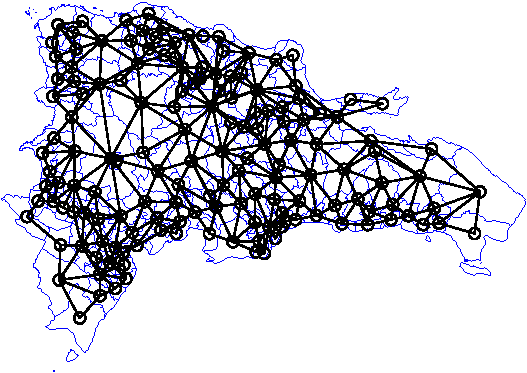
\includegraphics{proyecto_files/figure-latex/unnamed-chunk-3-1.pdf}

Luego se asignan los pesos a cada relación vecina, lo que permitirá
definir la fuerza de esta relación en base a cercanía, obteniendo los
siguientes datos:

Estilo Weighted:

\begin{verbatim}
## Characteristics of weights list object:
## Neighbour list object:
## Number of regions: 155 
## Number of nonzero links: 804 
## Percentage nonzero weights: 3.346514 
## Average number of links: 5.187097 
## 
## Weights style: W 
## Weights constants summary:
##     n    nn  S0       S1       S2
## W 155 24025 155 65.94606 650.7687
\end{verbatim}

Estilo Binario:

\begin{verbatim}
## Characteristics of weights list object:
## Neighbour list object:
## Number of regions: 155 
## Number of nonzero links: 804 
## Percentage nonzero weights: 3.346514 
## Average number of links: 5.187097 
## 
## Weights style: B 
## Weights constants summary:
##     n    nn  S0   S1    S2
## B 155 24025 804 1608 19520
\end{verbatim}

Para evaluar la correlación se utilizó el índice I de Moran cuyos
resultados nos indican que existe correlación positiva, con una
expectativa de relación negativa.

\begin{verbatim}
## 
##  Moran I test under randomisation
## 
## data:  miobj$DISC_PCT  
## weights: miobj.w.W    
## 
## Moran I statistic standard deviate = 8.7034, p-value < 2.2e-16
## alternative hypothesis: greater
## sample estimates:
## Moran I statistic       Expectation          Variance 
##       0.440845006      -0.006493506       0.002641768
\end{verbatim}

En el gráfico de Moran podemos obervar los porcentajes de personas con
discapacidad, contra el valor esperado de los mismos con relación a su
ubicación espacial, obteniendo los datos de los municipios donde el
porcentaje no se relaciona con sus vecinos.

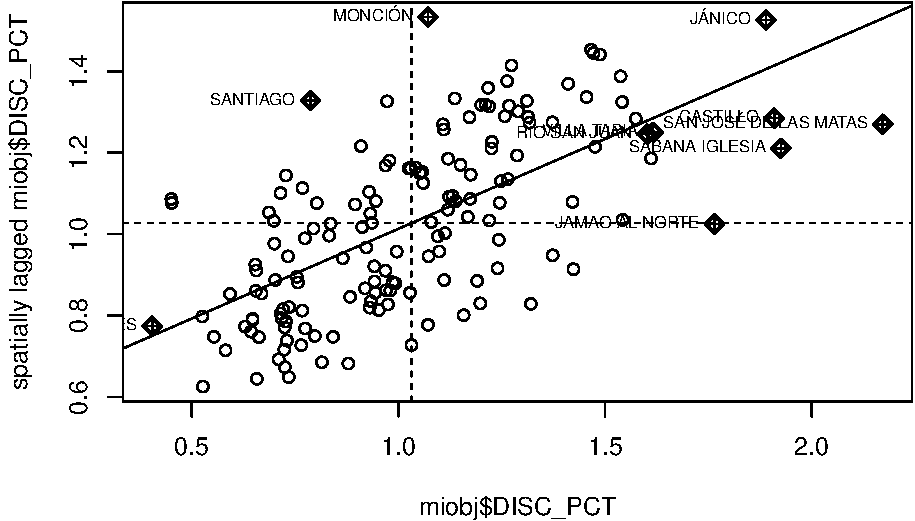
\includegraphics{proyecto_files/figure-latex/unnamed-chunk-7-1.pdf}

Para obtener el mapa que nos entregue información sobre los patrones
geográficos de autocorrelación espacial, realizamos un mapa LISA (Local
indicator of spatial asociation), donde podemos visualizar los clusters
de personas con discapacidad en la República Dominicana. Al mismo
tiempo, identifica los municipios donde la medición de la variable
corresponde a valores inferiores al promedio, rodeados por municipios
vecinos que también se encuentran bajo la media en relación al
porcentaje de discapacidad (cold spots).

\begin{verbatim}
## $grafico
\end{verbatim}

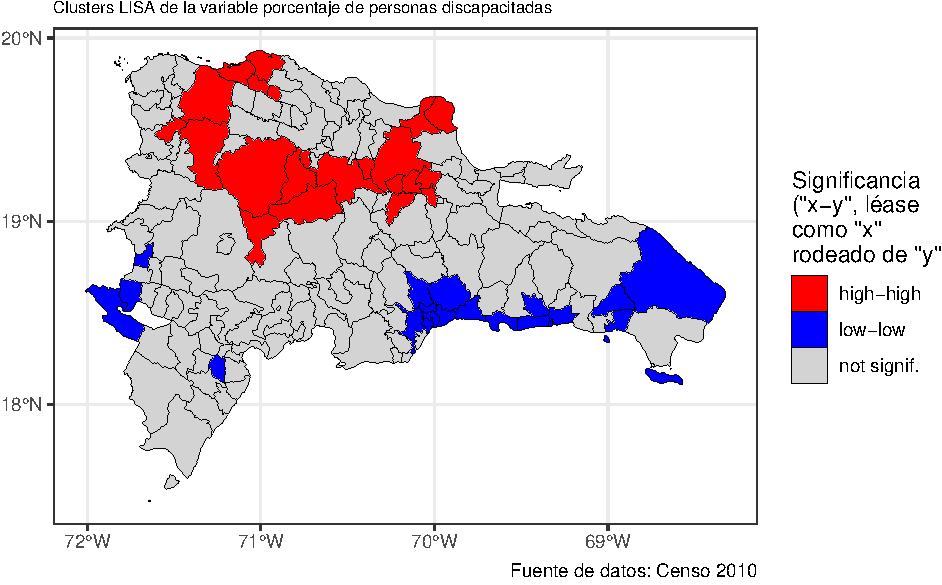
\includegraphics{proyecto_files/figure-latex/unnamed-chunk-9-1.pdf}

\begin{verbatim}
## 
## $objeto
## Simple feature collection with 155 features and 22 fields
## geometry type:  MULTIPOLYGON
## dimension:      XY
## bbox:           xmin: -72.01147 ymin: 17.47033 xmax: -68.32354 ymax: 19.93211
## epsg (SRID):    4326
## proj4string:    +proj=longlat +datum=WGS84 +no_defs
## First 10 features:
##                  TOPONIMIA Contaminación: Aguas estancadas: Si
## 1  SANTO DOMINGO DE GUZMÁN                              105331
## 2                     AZUA                                6354
## 3              LAS CHARCAS                                 840
## 4     LAS YAYAS DE VIAJAMA                                 490
## 5          PADRE LAS CASAS                                1773
## 6                  PERALTA                                   0
## 7             SABANA YEGUA                                   0
## 8             PUEBLO VIEJO                                 904
## 9            TÁBARA ARRIBA                                 417
## 10                GUAYABAL                                   0
##    Contaminación: Basura: Si Contaminación: Cañada: Si
## 1                     118868                     69359
## 2                       8873                      6987
## 3                        788                       458
## 4                       2509                      1216
## 5                        882                      3132
## 6                        102                       936
## 7                        648                        59
## 8                       1244                       955
## 9                        675                       587
## 10                         0                       123
##    Contaminación: Pocilga o granja: Si
## 1                                31519
## 2                                 4440
## 3                                    0
## 4                                    0
## 5                                  278
## 6                                    0
## 7                                    0
## 8                                   50
## 9                                    0
## 10                                   0
##    Contaminación: Humo o gases de fábrica: Si
## 1                                       31519
## 2                                        4440
## 3                                           0
## 4                                           0
## 5                                         278
## 6                                           0
## 7                                           0
## 8                                          50
## 9                                           0
## 10                                          0
##    Contaminación: Desechos o residuos de fábrica, taller, hospital: Si
## 1                                                                31561
## 2                                                                 1831
## 3                                                                    0
## 4                                                                    0
## 5                                                                  389
## 6                                                                    0
## 7                                                                    0
## 8                                                                   50
## 9                                                                    0
## 10                                                                   0
##    Contaminación: Envasadora de gas: Si Contaminación: Bomba gasolina: Si
## 1                                 26655                             32515
## 2                                  2496                              2268
## 3                                   103                                 0
## 4                                     0                                 0
## 5                                   232                                 0
## 6                                     0                                 0
## 7                                     0                                 0
## 8                                   456                                50
## 9                                   116                                 0
## 10                                    0                                 0
##    Contaminación: Fábrica productos químicos: Si
## 1                                          17444
## 2                                           1015
## 3                                              0
## 4                                            127
## 5                                              0
## 6                                              0
## 7                                              0
## 8                                            195
## 9                                              0
## 10                                             0
##    Contaminación: Ruído de vehículos y motores: Si
## 1                                           174313
## 2                                            14641
## 3                                             1669
## 4                                             2914
## 5                                             3509
## 6                                             2813
## 7                                             4699
## 8                                              459
## 9                                             1044
## 10                                            1171
##    Contaminación: Ruídos de fábrica o taller: Si
## 1                                          60971
## 2                                           4884
## 3                                              0
## 4                                             89
## 5                                            274
## 6                                              0
## 7                                              0
## 8                                            253
## 9                                              0
## 10                                             0
##    Contaminación: Ruídos o humo de planta eléctrica: Si
## 1                                                 64207
## 2                                                  5554
## 3                                                   318
## 4                                                     0
## 5                                                   642
## 6                                                  1996
## 7                                                  4699
## 8                                                     0
## 9                                                     0
## 10                                                    0
##    Contaminación: Música alta de bares, colmados o vecinos: Si
## 1                                                       134907
## 2                                                        11982
## 3                                                         1455
## 4                                                         2773
## 5                                                         2758
## 6                                                         2166
## 7                                                         5229
## 8                                                         1154
## 9                                                         1698
## 10                                                         181
##    Contaminación: Otra: Si TOTALPERS DISC TOTALVIV
## 1                    65854    965040 6344   330562
## 2                     7785     91345  597    24717
## 3                      692     11243   87     4091
## 4                      910     17620  140     5605
## 5                     2301     20041  225     6588
## 6                       84     15257  148     3590
## 7                       59     19020  168     5422
## 8                      203     11235   87     2897
## 9                      701     17647  196     4534
## 10                       0      5263   44     1850
##                              geom  DISC_PCT puntuacionz lagpuntuacionz
## 1  MULTIPOLYGON (((-69.89794 1... 0.6573821  -1.1667143    -1.20554715
## 2  MULTIPOLYGON (((-70.71457 1... 0.6535662  -1.1786151    -0.33091336
## 3  MULTIPOLYGON (((-70.50185 1... 0.7738148  -0.8035935    -0.12983056
## 4  MULTIPOLYGON (((-70.85774 1... 0.7945516  -0.7389212    -0.05413897
## 5  MULTIPOLYGON (((-70.77551 1... 1.1226985   0.2844759     0.18881093
## 6  MULTIPOLYGON (((-70.73131 1... 0.9700465  -0.1916023    -0.52776837
## 7  MULTIPOLYGON (((-70.83014 1... 0.8832808  -0.4622002    -0.57784218
## 8  MULTIPOLYGON (((-70.79387 1... 0.7743658  -0.8018751    -0.82040765
## 9  MULTIPOLYGON (((-70.83352 1... 1.1106704   0.2469636    -0.44911605
## 10 MULTIPOLYGON (((-70.68664 1... 0.8360251  -0.6095773    -0.01742264
##       quad_sig
## 1      low-low
## 2  not signif.
## 3  not signif.
## 4  not signif.
## 5  not signif.
## 6  not signif.
## 7  not signif.
## 8  not signif.
## 9  not signif.
## 10 not signif.
\end{verbatim}

Para establecer la relación entre la variable de Discapacidad contra las
variables de contaminación se realiza entonces la modelización de los
datos.

Evaluando la correlación:

\begin{verbatim}
## 
##  Moran I test under randomisation
## 
## data:  seleccionadas_PCT_LOG$DISC_PCT  
## weights: miobj.w.W    
## 
## Moran I statistic standard deviate = 8.7034, p-value < 2.2e-16
## alternative hypothesis: greater
## sample estimates:
## Moran I statistic       Expectation          Variance 
##       0.440845006      -0.006493506       0.002641768
\end{verbatim}

\begin{verbatim}
## 
##  Moran I test under randomisation
## 
## data:  seleccionadas_PCT_LOG$DISC_PCT  
## weights: miobj.w.B    
## 
## Moran I statistic standard deviate = 8.4261, p-value < 2.2e-16
## alternative hypothesis: greater
## sample estimates:
## Moran I statistic       Expectation          Variance 
##       0.403333528      -0.006493506       0.002365620
\end{verbatim}

\begin{verbatim}
## 
##  Moran I test under randomisation
## 
## data:  seleccionadas_PCT_LOG$DISC_PCT_LOG  
## weights: miobj.w.W    
## 
## Moran I statistic standard deviate = 8.8736, p-value < 2.2e-16
## alternative hypothesis: greater
## sample estimates:
## Moran I statistic       Expectation          Variance 
##       0.450717588      -0.006493506       0.002654817
\end{verbatim}

\begin{verbatim}
## 
##  Moran I test under randomisation
## 
## data:  seleccionadas_PCT_LOG$DISC_PCT_LOG  
## weights: miobj.w.B    
## 
## Moran I statistic standard deviate = 8.5397, p-value < 2.2e-16
## alternative hypothesis: greater
## sample estimates:
## Moran I statistic       Expectation          Variance 
##       0.409873887      -0.006493506       0.002377199
\end{verbatim}

Todos los resultados muestran correlación positiva y valores de p
menores que el nivel de significancia de 0.05, por lo que se puede
rechazar la hipótesis nula e indicar que existe correlación entre las
variables.

Evaluando el supuesto de normalidad:

\begin{verbatim}
## 
##  Shapiro-Wilk normality test
## 
## data:  seleccionadas_PCT_LOG$DISC_PCT
## W = 0.96682, p-value = 0.0008688
\end{verbatim}

\begin{verbatim}
## 
##  Shapiro-Wilk normality test
## 
## data:  seleccionadas_PCT_LOG$DISC_PCT_LOG
## W = 0.9888, p-value = 0.2528
\end{verbatim}

El test no nos da las evidencias suficientes para rechazar la hipótesis
de normalidad.

Contruyendo el modelo lineal:

\begin{verbatim}
## 
## Call:
## lm(formula = DISC_PCT_LOG ~ ., data = .)
## 
## Residuals:
##      Min       1Q   Median       3Q      Max 
## -0.32231 -0.10425 -0.00322  0.09114  0.43537 
## 
## Coefficients:
##                                            Estimate Std. Error t value
## (Intercept)                                0.658056   0.073672   8.932
## AguaEstancada_PCT_LOG                      0.006772   0.016578   0.408
## Basura_PCT_LOG                            -0.051129   0.017596  -2.906
## Cañada_PCT_LOG                             0.058492   0.017111   3.418
## Pocilga_Granja_PCT_LOG                    -0.121041   0.074456  -1.626
## Humo_GasesFábrica_PCT_LOG                  0.111520   0.075453   1.478
## Desechos_Fabrica_Taller_Hospital_PCT_LOG  -0.011363   0.020412  -0.557
## EnvasadoraGas_PCT_LOG                      0.022767   0.015310   1.487
## BombaGasolina_PCT_LOG                      0.008719   0.017739   0.492
## Fabrica_ProductosQuimicos_PCT_LOG         -0.052529   0.021165  -2.482
## Ruido_VehiculosyMotores_PCT_LOG            0.024714   0.024219   1.020
## Ruido_Fabrica_Taller_PCT_LOG               0.010089   0.017554   0.575
## RuidoYHumo_PlantaElectrica_PCT_LOG        -0.001338   0.013768  -0.097
## MusicaAlta_Bares_Colmados_Vecinos_PCT_LOG -0.024880   0.021866  -1.138
##                                           Pr(>|t|)    
## (Intercept)                               2.05e-15 ***
## AguaEstancada_PCT_LOG                     0.683532    
## Basura_PCT_LOG                            0.004256 ** 
## Cañada_PCT_LOG                            0.000824 ***
## Pocilga_Granja_PCT_LOG                    0.106250    
## Humo_GasesFábrica_PCT_LOG                 0.141639    
## Desechos_Fabrica_Taller_Hospital_PCT_LOG  0.578637    
## EnvasadoraGas_PCT_LOG                     0.139227    
## BombaGasolina_PCT_LOG                     0.623827    
## Fabrica_ProductosQuimicos_PCT_LOG         0.014245 *  
## Ruido_VehiculosyMotores_PCT_LOG           0.309259    
## Ruido_Fabrica_Taller_PCT_LOG              0.566378    
## RuidoYHumo_PlantaElectrica_PCT_LOG        0.922714    
## MusicaAlta_Bares_Colmados_Vecinos_PCT_LOG 0.257119    
## ---
## Signif. codes:  0 '***' 0.001 '**' 0.01 '*' 0.05 '.' 0.1 ' ' 1
## 
## Residual standard error: 0.1437 on 141 degrees of freedom
## Multiple R-squared:  0.2038, Adjusted R-squared:  0.1304 
## F-statistic: 2.776 on 13 and 141 DF,  p-value: 0.00151
\end{verbatim}

Resultan significativas las variables de contaminación por Basura,
Cañada y Fábrica de productos químicos.

Evaluando la heterocedasticidad:

\begin{verbatim}
## 
##  studentized Breusch-Pagan test
## 
## data:  .
## BP = 8.2401, df = 13, p-value = 0.8276
\end{verbatim}

Con un valor de p mayor de 0.05, no podemos rechazar la hipótesis nula.
Por lo tanto suponemos homogeneidad de varianzas.

Contruyendo el modelo espacial autorregresivo:

\begin{verbatim}
## Warning: Method summary.spautolm moved to the spatialreg package
\end{verbatim}

\begin{verbatim}
## Warning in summary.spautolm(sar2): install the spatialreg package
\end{verbatim}

\begin{verbatim}
## Warning: Method LR1.spautolm moved to the spatialreg package
\end{verbatim}

\begin{verbatim}
## Warning in LR1.spautolm(object): install the spatialreg package
\end{verbatim}

\begin{verbatim}
## Warning: Method logLik.spautolm moved to the spatialreg package
\end{verbatim}

\begin{verbatim}
## Warning in logLik.spautolm(object): install the spatialreg package
\end{verbatim}

\begin{verbatim}
## Warning: Method print.summary.spautolm moved to the spatialreg package
\end{verbatim}

\begin{verbatim}
## Warning in print.summary.spautolm(x): install the spatialreg package
\end{verbatim}

\begin{verbatim}
## 
## Call: 
## spautolm(formula = DISC_PCT_LOG ~ Basura_PCT_LOG + Cañada_PCT_LOG + 
##     Fabrica_ProductosQuimicos_PCT_LOG, data = ., listw = miobj.w.W)
## 
## Residuals:
\end{verbatim}

\begin{verbatim}
## Warning: Method residuals.spautolm moved to the spatialreg package
\end{verbatim}

\begin{verbatim}
## Warning in residuals.spautolm(x): install the spatialreg package
\end{verbatim}

\begin{verbatim}
##        Min         1Q     Median         3Q        Max 
## -0.3688384 -0.0657925 -0.0039986  0.0692903  0.3852568 
## 
## Coefficients: 
##                                    Estimate Std. Error z value  Pr(>|z|)
## (Intercept)                        0.707040   0.043217 16.3601 < 2.2e-16
## Basura_PCT_LOG                    -0.027990   0.013091 -2.1381  0.032510
## Cañada_PCT_LOG                     0.033893   0.012098  2.8015  0.005086
## Fabrica_ProductosQuimicos_PCT_LOG -0.038521   0.016172 -2.3820  0.017219
## 
## Lambda: 0.65067 LR test value: 47.328 p-value: 6.006e-12 
## Numerical Hessian standard error of lambda: 0.07417
\end{verbatim}

\begin{verbatim}
## Warning: Method logLik.spautolm moved to the spatialreg package
\end{verbatim}

\begin{verbatim}
## Warning in logLik.spautolm(x): install the spatialreg package
\end{verbatim}

\begin{verbatim}
## 
## Log likelihood: 107.035 
## ML residual variance (sigma squared): 0.013224, (sigma: 0.115)
## Number of observations: 155 
## Number of parameters estimated: 6
\end{verbatim}

\begin{verbatim}
## Warning: Method logLik.spautolm moved to the spatialreg package
\end{verbatim}

\begin{verbatim}
## Warning in logLik.spautolm(object): install the spatialreg package
\end{verbatim}

\begin{verbatim}
## AIC: -202.07
\end{verbatim}

Los coeficientes de regresión son 0.707 y 0.043. Podemos decir que 0.707
es el valor medio de la variable discapacidad cuando las variables
predictoras son cero. Mientras que 0.043, es el efecto medio sobre la
variable discapacidad al aumentar en una unidad el valor de las
variables de contaminación.

Existe una relación lineal positiva entre las variables, cuando aumentan
en una unidad las variables de contaminación, la discapacidad aumenta en
0.043 unidades.

Para finalizar se muestran los resultados del análisis geoestadístico en
un mapa donde se puede visualizar la cantidad de precipitaciones en el
país durante al año 1984:

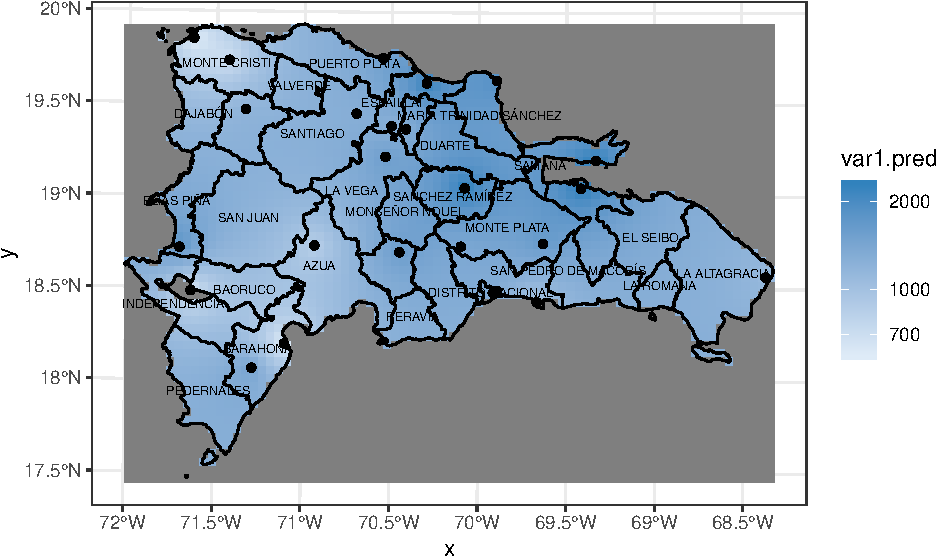
\includegraphics{proyecto_files/figure-latex/unnamed-chunk-19-1.pdf}

\section{Información de soporte}\label{informaciuxf3n-de-soporte}

Libro Análisis espacial con R: Usa R como un Sistema de Información
Geográfica, Jean-François Mas. Repositorio Material de Apoyo en GitHub.

\section{\texorpdfstring{\emph{Script}
reproducible}{Script reproducible}}\label{script-reproducible}

\section{Carga de los paquetes
necesarios}\label{carga-de-los-paquetes-necesarios}

\begin{Shaded}
\begin{Highlighting}[]
\KeywordTok{library}\NormalTok{(sf)}
\KeywordTok{library}\NormalTok{(raster)}
\KeywordTok{library}\NormalTok{(rgdal)}
\KeywordTok{library}\NormalTok{(tidyverse)}
\KeywordTok{library}\NormalTok{(readxl)}
\KeywordTok{library}\NormalTok{(tmap)}
\KeywordTok{library}\NormalTok{(RColorBrewer)}
\KeywordTok{library}\NormalTok{(units)}
\KeywordTok{library}\NormalTok{(spdep)}
\KeywordTok{library}\NormalTok{(lmtest)}
\KeywordTok{library}\NormalTok{(ggplot2)}
\KeywordTok{library}\NormalTok{(gstat)}
\KeywordTok{library}\NormalTok{(stars)}
\KeywordTok{source}\NormalTok{(}\StringTok{'lisaclusters.R'}\NormalTok{)}
\end{Highlighting}
\end{Shaded}

\section{Analisis Exploratorio de los
Datos}\label{analisis-exploratorio-de-los-datos}

\begin{Shaded}
\begin{Highlighting}[]
\NormalTok{vivpersgeom_sf <-}\StringTok{ }\KeywordTok{readRDS}\NormalTok{(}\StringTok{'DATA/vivpersgeom_sf.RDS'}\NormalTok{)}
\NormalTok{miobj <-}\StringTok{ }\NormalTok{vivpersgeom_sf }\OperatorTok\StringTok{ }\KeywordTok{select}\NormalTok{(}
  \KeywordTok{matches}\NormalTok{(}\StringTok{'TOPONIMIA|Categoría Ocupacional: Discapacitado|Contaminación.*Si$|Población total|Condición de ocupación')}
\StringTok{)}
\StringTok{miobj <- miobj %>% mutate(TOTALVIV=`Condición de ocupación: Ocupada con personas presentes` + `Condición de ocupación: Desocupada`) %>% select(-matches('}\NormalTok{Condición de ocupación'))}
\NormalTok{miobj <-}\StringTok{ }\NormalTok{miobj }\OperatorTok\StringTok{ }\KeywordTok{rename}\NormalTok{(}\DataTypeTok{TOTALPERS=}\StringTok{'Población total'}\NormalTok{, }\DataTypeTok{DISC=}\StringTok{'Categoría Ocupacional: Discapacitado'}\NormalTok{) }\OperatorTok\StringTok{ }\KeywordTok{mutate}\NormalTok{(}\DataTypeTok{DISC_PCT=}\NormalTok{DISC}\OperatorTok{/}\NormalTok{TOTALPERS}\OperatorTok{*}\DecValTok{100}\NormalTok{)}
\NormalTok{miobj}
\end{Highlighting}
\end{Shaded}

\begin{verbatim}
## Simple feature collection with 155 features and 19 fields
## geometry type:  MULTIPOLYGON
## dimension:      XY
## bbox:           xmin: -72.01147 ymin: 17.47033 xmax: -68.32354 ymax: 19.93211
## epsg (SRID):    4326
## proj4string:    +proj=longlat +datum=WGS84 +no_defs
## First 10 features:
##                  TOPONIMIA Contaminación: Aguas estancadas: Si
## 1  SANTO DOMINGO DE GUZMÁN                              105331
## 2                     AZUA                                6354
## 3              LAS CHARCAS                                 840
## 4     LAS YAYAS DE VIAJAMA                                 490
## 5          PADRE LAS CASAS                                1773
## 6                  PERALTA                                   0
## 7             SABANA YEGUA                                   0
## 8             PUEBLO VIEJO                                 904
## 9            TÁBARA ARRIBA                                 417
## 10                GUAYABAL                                   0
##    Contaminación: Basura: Si Contaminación: Cañada: Si
## 1                     118868                     69359
## 2                       8873                      6987
## 3                        788                       458
## 4                       2509                      1216
## 5                        882                      3132
## 6                        102                       936
## 7                        648                        59
## 8                       1244                       955
## 9                        675                       587
## 10                         0                       123
##    Contaminación: Pocilga o granja: Si
## 1                                31519
## 2                                 4440
## 3                                    0
## 4                                    0
## 5                                  278
## 6                                    0
## 7                                    0
## 8                                   50
## 9                                    0
## 10                                   0
##    Contaminación: Humo o gases de fábrica: Si
## 1                                       31519
## 2                                        4440
## 3                                           0
## 4                                           0
## 5                                         278
## 6                                           0
## 7                                           0
## 8                                          50
## 9                                           0
## 10                                          0
##    Contaminación: Desechos o residuos de fábrica, taller, hospital: Si
## 1                                                                31561
## 2                                                                 1831
## 3                                                                    0
## 4                                                                    0
## 5                                                                  389
## 6                                                                    0
## 7                                                                    0
## 8                                                                   50
## 9                                                                    0
## 10                                                                   0
##    Contaminación: Envasadora de gas: Si Contaminación: Bomba gasolina: Si
## 1                                 26655                             32515
## 2                                  2496                              2268
## 3                                   103                                 0
## 4                                     0                                 0
## 5                                   232                                 0
## 6                                     0                                 0
## 7                                     0                                 0
## 8                                   456                                50
## 9                                   116                                 0
## 10                                    0                                 0
##    Contaminación: Fábrica productos químicos: Si
## 1                                          17444
## 2                                           1015
## 3                                              0
## 4                                            127
## 5                                              0
## 6                                              0
## 7                                              0
## 8                                            195
## 9                                              0
## 10                                             0
##    Contaminación: Ruído de vehículos y motores: Si
## 1                                           174313
## 2                                            14641
## 3                                             1669
## 4                                             2914
## 5                                             3509
## 6                                             2813
## 7                                             4699
## 8                                              459
## 9                                             1044
## 10                                            1171
##    Contaminación: Ruídos de fábrica o taller: Si
## 1                                          60971
## 2                                           4884
## 3                                              0
## 4                                             89
## 5                                            274
## 6                                              0
## 7                                              0
## 8                                            253
## 9                                              0
## 10                                             0
##    Contaminación: Ruídos o humo de planta eléctrica: Si
## 1                                                 64207
## 2                                                  5554
## 3                                                   318
## 4                                                     0
## 5                                                   642
## 6                                                  1996
## 7                                                  4699
## 8                                                     0
## 9                                                     0
## 10                                                    0
##    Contaminación: Música alta de bares, colmados o vecinos: Si
## 1                                                       134907
## 2                                                        11982
## 3                                                         1455
## 4                                                         2773
## 5                                                         2758
## 6                                                         2166
## 7                                                         5229
## 8                                                         1154
## 9                                                         1698
## 10                                                         181
##    Contaminación: Otra: Si TOTALPERS DISC TOTALVIV
## 1                    65854    965040 6344   330562
## 2                     7785     91345  597    24717
## 3                      692     11243   87     4091
## 4                      910     17620  140     5605
## 5                     2301     20041  225     6588
## 6                       84     15257  148     3590
## 7                       59     19020  168     5422
## 8                      203     11235   87     2897
## 9                      701     17647  196     4534
## 10                       0      5263   44     1850
##                              geom  DISC_PCT
## 1  MULTIPOLYGON (((-69.89794 1... 0.6573821
## 2  MULTIPOLYGON (((-70.71457 1... 0.6535662
## 3  MULTIPOLYGON (((-70.50185 1... 0.7738148
## 4  MULTIPOLYGON (((-70.85774 1... 0.7945516
## 5  MULTIPOLYGON (((-70.77551 1... 1.1226985
## 6  MULTIPOLYGON (((-70.73131 1... 0.9700465
## 7  MULTIPOLYGON (((-70.83014 1... 0.8832808
## 8  MULTIPOLYGON (((-70.79387 1... 0.7743658
## 9  MULTIPOLYGON (((-70.83352 1... 1.1106704
## 10 MULTIPOLYGON (((-70.68664 1... 0.8360251
\end{verbatim}

\begin{Shaded}
\begin{Highlighting}[]
\NormalTok{rutadiv <-}\StringTok{ 'DATA/divisionRD.gpkg'}
\NormalTok{prov <-}\StringTok{ }\KeywordTok{st_read}\NormalTok{(rutadiv, }\DataTypeTok{layer =} \StringTok{'PROVCenso2010'}\NormalTok{)}
\end{Highlighting}
\end{Shaded}

\begin{verbatim}
## Reading layer `PROVCenso2010' from data source `/home/masue/unidad-0-asignacion-99-mi-proyecto-masuero/DATA/divisionRD.gpkg' using driver `GPKG'
## Simple feature collection with 32 features and 4 fields
## geometry type:  MULTIPOLYGON
## dimension:      XY
## bbox:           xmin: 182215.8 ymin: 1933532 xmax: 571365.3 ymax: 2205216
## epsg (SRID):    32619
## proj4string:    +proj=utm +zone=19 +datum=WGS84 +units=m +no_defs
\end{verbatim}

\section{Análisis de Vecindad}\label{anuxe1lisis-de-vecindad}

\begin{Shaded}
\begin{Highlighting}[]
\NormalTok{miobj.sp <-}\StringTok{ }\KeywordTok{as_Spatial}\NormalTok{(miobj)}
\NormalTok{miobj.nb <-}\StringTok{ }\KeywordTok{poly2nb}\NormalTok{(}\KeywordTok{as}\NormalTok{(miobj, }\StringTok{'Spatial'}\NormalTok{), }\DataTypeTok{row.names =}\NormalTok{ miobj}\OperatorTok{$}\NormalTok{TOPONIMIA, }\DataTypeTok{queen =} \OtherTok{TRUE}\NormalTok{)}
\KeywordTok{summary}\NormalTok{(miobj.nb)}
\end{Highlighting}
\end{Shaded}

\begin{verbatim}
## Neighbour list object:
## Number of regions: 155 
## Number of nonzero links: 804 
## Percentage nonzero weights: 3.346514 
## Average number of links: 5.187097 
## Link number distribution:
## 
##  1  2  3  4  5  6  7  8  9 10 11 12 14 
##  1 10 20 34 33 22 13 13  4  1  1  2  1 
## 1 least connected region:
## JUAN DE HERRERA with 1 link
## 1 most connected region:
## LA VEGA with 14 links
\end{verbatim}

\begin{Shaded}
\begin{Highlighting}[]
\NormalTok{coords <-}\StringTok{ }\KeywordTok{coordinates}\NormalTok{(}\KeywordTok{as}\NormalTok{((miobj), }\StringTok{'Spatial'}\NormalTok{))}
\KeywordTok{plot}\NormalTok{(miobj.sp, }\DataTypeTok{border=}\StringTok{"blue"}\NormalTok{, }\DataTypeTok{lwd=}\FloatTok{0.5}\NormalTok{)}
\KeywordTok{plot.nb}\NormalTok{(miobj.nb,coords, }\DataTypeTok{add =}\NormalTok{ T)}
\end{Highlighting}
\end{Shaded}

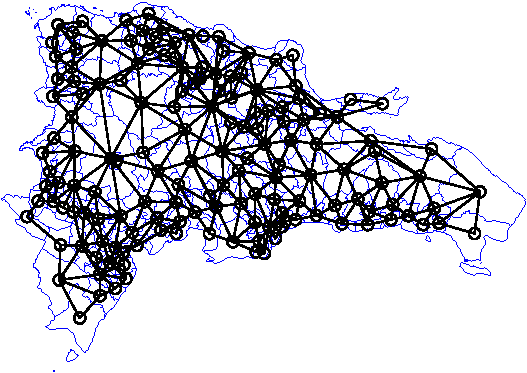
\includegraphics{proyecto_files/figure-latex/unnamed-chunk-22-1.pdf}

\section{Matriz de Pesos Espaciales}\label{matriz-de-pesos-espaciales}

\begin{Shaded}
\begin{Highlighting}[]
\NormalTok{miobj.w.W <-}\StringTok{ }\KeywordTok{nb2listw}\NormalTok{(miobj.nb)}
\NormalTok{miobj.w.W}
\end{Highlighting}
\end{Shaded}

\begin{verbatim}
## Characteristics of weights list object:
## Neighbour list object:
## Number of regions: 155 
## Number of nonzero links: 804 
## Percentage nonzero weights: 3.346514 
## Average number of links: 5.187097 
## 
## Weights style: W 
## Weights constants summary:
##     n    nn  S0       S1       S2
## W 155 24025 155 65.94606 650.7687
\end{verbatim}

\begin{Shaded}
\begin{Highlighting}[]
\NormalTok{miobj.w.B <-}\StringTok{ }\KeywordTok{nb2listw}\NormalTok{(miobj.nb, }\DataTypeTok{style =} \StringTok{'B'}\NormalTok{)}
\NormalTok{miobj.w.B}
\end{Highlighting}
\end{Shaded}

\begin{verbatim}
## Characteristics of weights list object:
## Neighbour list object:
## Number of regions: 155 
## Number of nonzero links: 804 
## Percentage nonzero weights: 3.346514 
## Average number of links: 5.187097 
## 
## Weights style: B 
## Weights constants summary:
##     n    nn  S0   S1    S2
## B 155 24025 804 1608 19520
\end{verbatim}

\section{Test de I de Moran Global}\label{test-de-i-de-moran-global}

\begin{Shaded}
\begin{Highlighting}[]
\KeywordTok{moran.test}\NormalTok{(miobj}\OperatorTok{$}\NormalTok{DISC, }\DataTypeTok{listw =}\NormalTok{ miobj.w.W)}
\end{Highlighting}
\end{Shaded}

\begin{verbatim}
## 
##  Moran I test under randomisation
## 
## data:  miobj$DISC  
## weights: miobj.w.W    
## 
## Moran I statistic standard deviate = 7.0861, p-value = 6.895e-13
## alternative hypothesis: greater
## sample estimates:
## Moran I statistic       Expectation          Variance 
##       0.333118530      -0.006493506       0.002296919
\end{verbatim}

\begin{Shaded}
\begin{Highlighting}[]
\KeywordTok{moran.test}\NormalTok{(miobj}\OperatorTok{$}\NormalTok{DISC_PCT, }\DataTypeTok{listw =}\NormalTok{ miobj.w.W)}
\end{Highlighting}
\end{Shaded}

\begin{verbatim}
## 
##  Moran I test under randomisation
## 
## data:  miobj$DISC_PCT  
## weights: miobj.w.W    
## 
## Moran I statistic standard deviate = 8.7034, p-value < 2.2e-16
## alternative hypothesis: greater
## sample estimates:
## Moran I statistic       Expectation          Variance 
##       0.440845006      -0.006493506       0.002641768
\end{verbatim}

\begin{Shaded}
\begin{Highlighting}[]
\KeywordTok{moran.plot}\NormalTok{(miobj}\OperatorTok{$}\NormalTok{DISC, }\DataTypeTok{listw =}\NormalTok{ miobj.w.W)}
\end{Highlighting}
\end{Shaded}

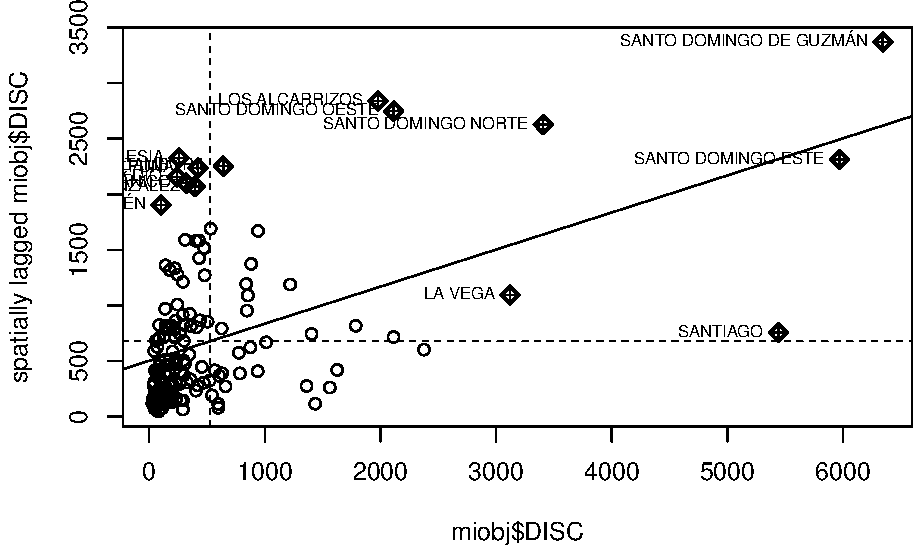
\includegraphics{proyecto_files/figure-latex/unnamed-chunk-24-1.pdf}

\begin{Shaded}
\begin{Highlighting}[]
\KeywordTok{moran.plot}\NormalTok{(miobj}\OperatorTok{$}\NormalTok{DISC_PCT, }\DataTypeTok{listw =}\NormalTok{ miobj.w.W)}
\end{Highlighting}
\end{Shaded}

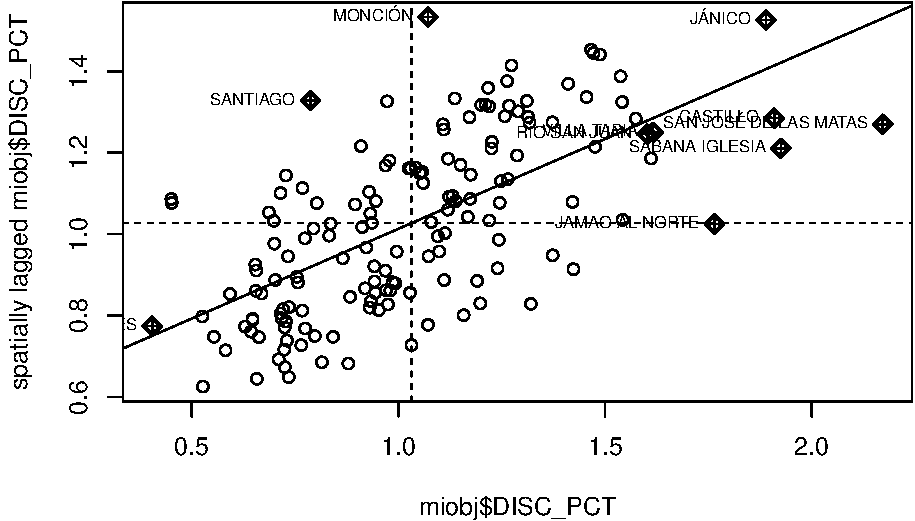
\includegraphics{proyecto_files/figure-latex/unnamed-chunk-24-2.pdf}

\section{Test de I de Moran Local}\label{test-de-i-de-moran-local}

\begin{Shaded}
\begin{Highlighting}[]
\NormalTok{DISC_lmoran <-}\StringTok{ }\KeywordTok{localmoran}\NormalTok{(miobj}\OperatorTok{$}\NormalTok{DISC, }\DataTypeTok{listw =}\NormalTok{ miobj.w.W)}
\KeywordTok{summary}\NormalTok{(DISC_lmoran)}
\end{Highlighting}
\end{Shaded}

\begin{verbatim}
##        Ii                E.Ii               Var.Ii       
##  Min.   :-0.66810   Min.   :-0.006494   Min.   :0.05682  
##  1st Qu.:-0.05333   1st Qu.:-0.006494   1st Qu.:0.13880  
##  Median : 0.04040   Median :-0.006494   Median :0.16749  
##  Mean   : 0.33312   Mean   :-0.006494   Mean   :0.19408  
##  3rd Qu.: 0.16302   3rd Qu.:-0.006494   3rd Qu.:0.21052  
##  Max.   :18.84791   Max.   :-0.006494   Max.   :0.85605  
##       Z.Ii           Pr(z > 0)     
##  Min.   :-1.2453   Min.   :0.0000  
##  1st Qu.:-0.1090   1st Qu.:0.3512  
##  Median : 0.1197   Median :0.4524  
##  Mean   : 0.8482   Mean   :0.4423  
##  3rd Qu.: 0.3821   3rd Qu.:0.5434  
##  Max.   :41.0927   Max.   :0.8935
\end{verbatim}

\begin{Shaded}
\begin{Highlighting}[]
\NormalTok{DISC_PCT_lmoran <-}\StringTok{ }\KeywordTok{localmoran}\NormalTok{(miobj}\OperatorTok{$}\NormalTok{DISC_PCT, }\DataTypeTok{listw =}\NormalTok{ miobj.w.W)}
\KeywordTok{summary}\NormalTok{(DISC_PCT_lmoran)}
\end{Highlighting}
\end{Shaded}

\begin{verbatim}
##        Ii                 E.Ii               Var.Ii       
##  Min.   :-0.709657   Min.   :-0.006494   Min.   :0.06436  
##  1st Qu.: 0.008281   1st Qu.:-0.006494   1st Qu.:0.15859  
##  Median : 0.187426   Median :-0.006494   Median :0.19157  
##  Mean   : 0.440845   Mean   :-0.006494   Mean   :0.22214  
##  3rd Qu.: 0.750052   3rd Qu.:-0.006494   3rd Qu.:0.24104  
##  Max.   : 4.150895   Max.   :-0.006494   Max.   :0.98310  
##       Z.Ii            Pr(z > 0)      
##  Min.   :-2.54836   Min.   :0.00000  
##  1st Qu.: 0.03344   1st Qu.:0.04706  
##  Median : 0.49281   Median :0.31107  
##  Mean   : 0.97963   Mean   :0.29895  
##  3rd Qu.: 1.67411   3rd Qu.:0.48666  
##  Max.   : 9.49860   Max.   :0.99459
\end{verbatim}

\begin{Shaded}
\begin{Highlighting}[]
\NormalTok{mapa_moran <-}\StringTok{ }\KeywordTok{cbind}\NormalTok{(miobj, DISC_lmoran)}
\KeywordTok{ggplot}\NormalTok{(mapa_moran)}\OperatorTok{+}
\StringTok{  }\KeywordTok{geom_sf}\NormalTok{(}\KeywordTok{aes}\NormalTok{(}\DataTypeTok{fill =}\NormalTok{ Ii))}\OperatorTok{+}
\StringTok{  }\KeywordTok{labs}\NormalTok{(}\DataTypeTok{fill =} \StringTok{"Estadísitico Moran Local"}\NormalTok{)}
\end{Highlighting}
\end{Shaded}

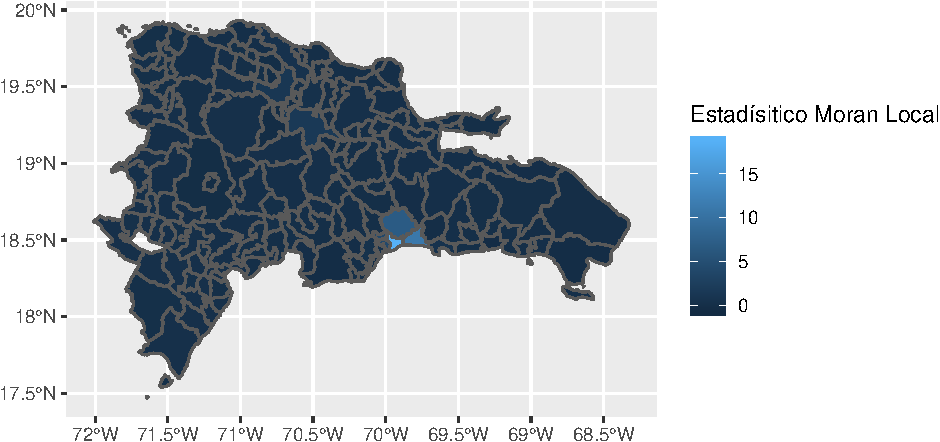
\includegraphics{proyecto_files/figure-latex/unnamed-chunk-25-1.pdf}

\begin{Shaded}
\begin{Highlighting}[]
\NormalTok{mapa_moran_DISC_PCT <-}\StringTok{ }\KeywordTok{cbind}\NormalTok{(miobj, DISC_PCT_lmoran)}
\KeywordTok{ggplot}\NormalTok{(mapa_moran_DISC_PCT)}\OperatorTok{+}
\StringTok{  }\KeywordTok{geom_sf}\NormalTok{(}\KeywordTok{aes}\NormalTok{(}\DataTypeTok{fill =}\NormalTok{ Ii))}\OperatorTok{+}
\StringTok{  }\KeywordTok{labs}\NormalTok{(}\DataTypeTok{fill =} \StringTok{"Estadísitico Moran Local"}\NormalTok{)}
\end{Highlighting}
\end{Shaded}

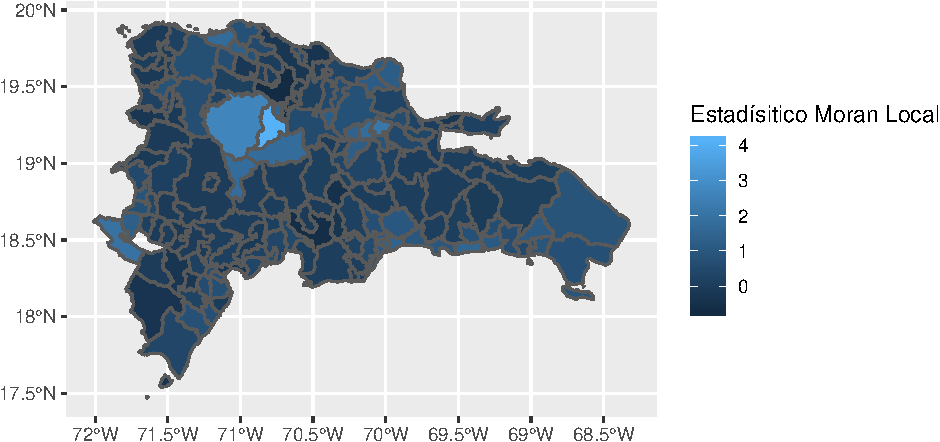
\includegraphics{proyecto_files/figure-latex/unnamed-chunk-25-2.pdf}

\section{Mapa de Cluster LISA}\label{mapa-de-cluster-lisa}

\begin{Shaded}
\begin{Highlighting}[]
\KeywordTok{lisamap}\NormalTok{(}\DataTypeTok{objesp =}\NormalTok{ miobj,}
        \DataTypeTok{var =} \StringTok{'DISC_PCT'}\NormalTok{,}
        \DataTypeTok{pesos =}\NormalTok{ miobj.w.W,}
        \DataTypeTok{tituloleyenda =} \StringTok{'Significancia}\CharTok{\textbackslash{}n}\StringTok{("x-y", léase}\CharTok{\textbackslash{}n}\StringTok{como "x"}\CharTok{\textbackslash{}n}\StringTok{rodeado de "y"'}\NormalTok{,}
        \DataTypeTok{leyenda =}\NormalTok{ T,}
        \DataTypeTok{anchuratitulo =} \DecValTok{700}\NormalTok{,}
        \DataTypeTok{tamanotitulo =} \DecValTok{8}\NormalTok{,}
        \DataTypeTok{fuentedatos =} \StringTok{'Censo 2010'}\NormalTok{,}
        \DataTypeTok{titulomapa =} \StringTok{'Clusters LISA de la variable porcentaje de personas discapacitadas'}\NormalTok{)}
\end{Highlighting}
\end{Shaded}

\begin{verbatim}
## $grafico
\end{verbatim}

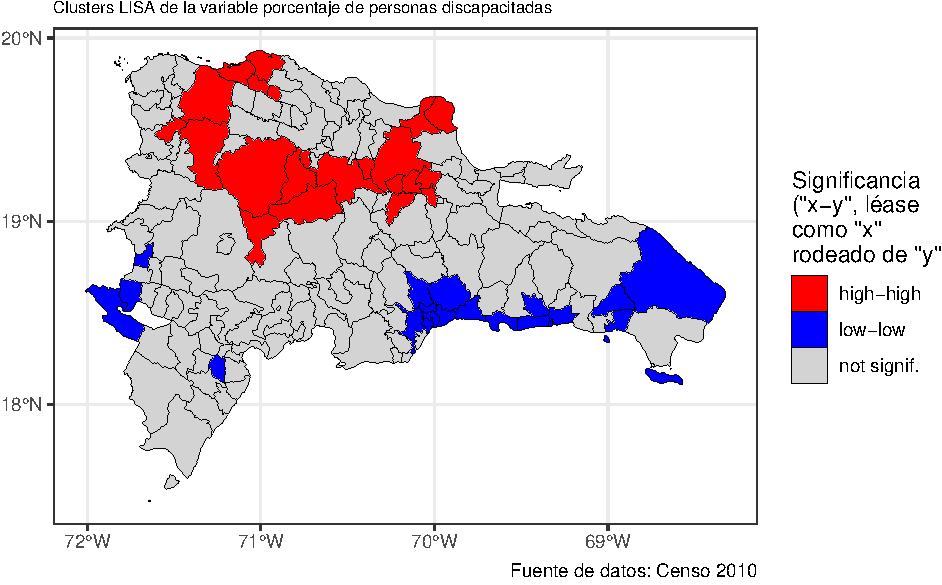
\includegraphics{proyecto_files/figure-latex/unnamed-chunk-26-1.pdf}

\begin{verbatim}
## 
## $objeto
## Simple feature collection with 155 features and 22 fields
## geometry type:  MULTIPOLYGON
## dimension:      XY
## bbox:           xmin: -72.01147 ymin: 17.47033 xmax: -68.32354 ymax: 19.93211
## epsg (SRID):    4326
## proj4string:    +proj=longlat +datum=WGS84 +no_defs
## First 10 features:
##                  TOPONIMIA Contaminación: Aguas estancadas: Si
## 1  SANTO DOMINGO DE GUZMÁN                              105331
## 2                     AZUA                                6354
## 3              LAS CHARCAS                                 840
## 4     LAS YAYAS DE VIAJAMA                                 490
## 5          PADRE LAS CASAS                                1773
## 6                  PERALTA                                   0
## 7             SABANA YEGUA                                   0
## 8             PUEBLO VIEJO                                 904
## 9            TÁBARA ARRIBA                                 417
## 10                GUAYABAL                                   0
##    Contaminación: Basura: Si Contaminación: Cañada: Si
## 1                     118868                     69359
## 2                       8873                      6987
## 3                        788                       458
## 4                       2509                      1216
## 5                        882                      3132
## 6                        102                       936
## 7                        648                        59
## 8                       1244                       955
## 9                        675                       587
## 10                         0                       123
##    Contaminación: Pocilga o granja: Si
## 1                                31519
## 2                                 4440
## 3                                    0
## 4                                    0
## 5                                  278
## 6                                    0
## 7                                    0
## 8                                   50
## 9                                    0
## 10                                   0
##    Contaminación: Humo o gases de fábrica: Si
## 1                                       31519
## 2                                        4440
## 3                                           0
## 4                                           0
## 5                                         278
## 6                                           0
## 7                                           0
## 8                                          50
## 9                                           0
## 10                                          0
##    Contaminación: Desechos o residuos de fábrica, taller, hospital: Si
## 1                                                                31561
## 2                                                                 1831
## 3                                                                    0
## 4                                                                    0
## 5                                                                  389
## 6                                                                    0
## 7                                                                    0
## 8                                                                   50
## 9                                                                    0
## 10                                                                   0
##    Contaminación: Envasadora de gas: Si Contaminación: Bomba gasolina: Si
## 1                                 26655                             32515
## 2                                  2496                              2268
## 3                                   103                                 0
## 4                                     0                                 0
## 5                                   232                                 0
## 6                                     0                                 0
## 7                                     0                                 0
## 8                                   456                                50
## 9                                   116                                 0
## 10                                    0                                 0
##    Contaminación: Fábrica productos químicos: Si
## 1                                          17444
## 2                                           1015
## 3                                              0
## 4                                            127
## 5                                              0
## 6                                              0
## 7                                              0
## 8                                            195
## 9                                              0
## 10                                             0
##    Contaminación: Ruído de vehículos y motores: Si
## 1                                           174313
## 2                                            14641
## 3                                             1669
## 4                                             2914
## 5                                             3509
## 6                                             2813
## 7                                             4699
## 8                                              459
## 9                                             1044
## 10                                            1171
##    Contaminación: Ruídos de fábrica o taller: Si
## 1                                          60971
## 2                                           4884
## 3                                              0
## 4                                             89
## 5                                            274
## 6                                              0
## 7                                              0
## 8                                            253
## 9                                              0
## 10                                             0
##    Contaminación: Ruídos o humo de planta eléctrica: Si
## 1                                                 64207
## 2                                                  5554
## 3                                                   318
## 4                                                     0
## 5                                                   642
## 6                                                  1996
## 7                                                  4699
## 8                                                     0
## 9                                                     0
## 10                                                    0
##    Contaminación: Música alta de bares, colmados o vecinos: Si
## 1                                                       134907
## 2                                                        11982
## 3                                                         1455
## 4                                                         2773
## 5                                                         2758
## 6                                                         2166
## 7                                                         5229
## 8                                                         1154
## 9                                                         1698
## 10                                                         181
##    Contaminación: Otra: Si TOTALPERS DISC TOTALVIV
## 1                    65854    965040 6344   330562
## 2                     7785     91345  597    24717
## 3                      692     11243   87     4091
## 4                      910     17620  140     5605
## 5                     2301     20041  225     6588
## 6                       84     15257  148     3590
## 7                       59     19020  168     5422
## 8                      203     11235   87     2897
## 9                      701     17647  196     4534
## 10                       0      5263   44     1850
##                              geom  DISC_PCT puntuacionz lagpuntuacionz
## 1  MULTIPOLYGON (((-69.89794 1... 0.6573821  -1.1667143    -1.20554715
## 2  MULTIPOLYGON (((-70.71457 1... 0.6535662  -1.1786151    -0.33091336
## 3  MULTIPOLYGON (((-70.50185 1... 0.7738148  -0.8035935    -0.12983056
## 4  MULTIPOLYGON (((-70.85774 1... 0.7945516  -0.7389212    -0.05413897
## 5  MULTIPOLYGON (((-70.77551 1... 1.1226985   0.2844759     0.18881093
## 6  MULTIPOLYGON (((-70.73131 1... 0.9700465  -0.1916023    -0.52776837
## 7  MULTIPOLYGON (((-70.83014 1... 0.8832808  -0.4622002    -0.57784218
## 8  MULTIPOLYGON (((-70.79387 1... 0.7743658  -0.8018751    -0.82040765
## 9  MULTIPOLYGON (((-70.83352 1... 1.1106704   0.2469636    -0.44911605
## 10 MULTIPOLYGON (((-70.68664 1... 0.8360251  -0.6095773    -0.01742264
##       quad_sig
## 1      low-low
## 2  not signif.
## 3  not signif.
## 4  not signif.
## 5  not signif.
## 6  not signif.
## 7  not signif.
## 8  not signif.
## 9  not signif.
## 10 not signif.
\end{verbatim}

\section{Modelización}\label{modelizaciuxf3n}

\begin{Shaded}
\begin{Highlighting}[]
\KeywordTok{names}\NormalTok{ (miobj)}
\end{Highlighting}
\end{Shaded}

\begin{verbatim}
##  [1] "TOPONIMIA"                                                          
##  [2] "Contaminación: Aguas estancadas: Si"                                
##  [3] "Contaminación: Basura: Si"                                          
##  [4] "Contaminación: Cañada: Si"                                          
##  [5] "Contaminación: Pocilga o granja: Si"                                
##  [6] "Contaminación: Humo o gases de fábrica: Si"                         
##  [7] "Contaminación: Desechos o residuos de fábrica, taller, hospital: Si"
##  [8] "Contaminación: Envasadora de gas: Si"                               
##  [9] "Contaminación: Bomba gasolina: Si"                                  
## [10] "Contaminación: Fábrica productos químicos: Si"                      
## [11] "Contaminación: Ruído de vehículos y motores: Si"                    
## [12] "Contaminación: Ruídos de fábrica o taller: Si"                      
## [13] "Contaminación: Ruídos o humo de planta eléctrica: Si"               
## [14] "Contaminación: Música alta de bares, colmados o vecinos: Si"        
## [15] "Contaminación: Otra: Si"                                            
## [16] "TOTALPERS"                                                          
## [17] "DISC"                                                               
## [18] "TOTALVIV"                                                           
## [19] "geom"                                                               
## [20] "DISC_PCT"
\end{verbatim}

\begin{Shaded}
\begin{Highlighting}[]
\NormalTok{seleccionadas <-}\StringTok{ }\NormalTok{miobj }\OperatorTok\StringTok{ }\NormalTok{dplyr}\OperatorTok{::}\KeywordTok{select}\NormalTok{(}
  \DataTypeTok{TOPONIMIA =}\NormalTok{ TOPONIMIA,}
  \DataTypeTok{DISC =}\NormalTok{ DISC,}
  \DataTypeTok{TOTALPERS =}\NormalTok{ TOTALPERS,}
  \DataTypeTok{TOTALVIV =}\NormalTok{ TOTALVIV,}
  \DataTypeTok{DISC_PCT =}\NormalTok{ DISC_PCT,}
  \DataTypeTok{AguaEstancada =} \StringTok{"Contaminación: Aguas estancadas: Si"}\NormalTok{,}
  \DataTypeTok{Basura =} \StringTok{"Contaminación: Basura: Si"}\NormalTok{,}
\NormalTok{  Cañ}\DataTypeTok{ada =} \StringTok{"Contaminación: Cañada: Si"}\NormalTok{,}
  \DataTypeTok{Pocilga_Granja =} \StringTok{"Contaminación: Pocilga o granja: Si"}\NormalTok{,}
\NormalTok{  Humo_GasesFá}\DataTypeTok{brica =} \StringTok{"Contaminación: Humo o gases de fábrica: Si"}\NormalTok{,}
  \DataTypeTok{Desechos_Fabrica_Taller_Hospital =} \StringTok{"Contaminación: Desechos o residuos de fábrica, taller, hospital: Si"}\NormalTok{,}
  \DataTypeTok{EnvasadoraGas =} \StringTok{"Contaminación: Envasadora de gas: Si"}\NormalTok{,}
  \DataTypeTok{BombaGasolina =} \StringTok{"Contaminación: Bomba gasolina: Si"}\NormalTok{,}
  \DataTypeTok{Fabrica_ProductosQuimicos =}  \StringTok{"Contaminación: Fábrica productos químicos: Si"}\NormalTok{,}
  \DataTypeTok{Ruido_VehiculosyMotores =} \StringTok{"Contaminación: Ruído de vehículos y motores: Si"}\NormalTok{,}
  \DataTypeTok{Ruido_Fabrica_Taller =} \StringTok{"Contaminación: Ruídos de fábrica o taller: Si"}\NormalTok{,}
  \DataTypeTok{RuidoYHumo_PlantaElectrica =} \StringTok{"Contaminación: Ruídos o humo de planta eléctrica: Si"}\NormalTok{,}
  \DataTypeTok{MusicaAlta_Bares_Colmados_Vecinos =} \StringTok{"Contaminación: Música alta de bares, colmados o vecinos: Si"}\NormalTok{)}
  

\NormalTok{seleccionadas_PCT <-}\StringTok{ }\NormalTok{seleccionadas }\OperatorTok\StringTok{ }\KeywordTok{mutate}\NormalTok{(}\DataTypeTok{AguaEstancada_PCT=}\NormalTok{ AguaEstancada}\OperatorTok{/}\NormalTok{TOTALVIV}\OperatorTok{*}\DecValTok{100}\NormalTok{, }\DataTypeTok{Basura_PCT=}\NormalTok{Basura}\OperatorTok{/}\NormalTok{TOTALVIV}\OperatorTok{*}\DecValTok{100}\NormalTok{, Cañ}\DataTypeTok{ada_PCT=}\NormalTok{Cañada}\OperatorTok{/}\NormalTok{TOTALVIV}\OperatorTok{*}\DecValTok{100}\NormalTok{, }\DataTypeTok{Pocilga_Granja_PCT=}\NormalTok{Pocilga_Granja}\OperatorTok{/}\NormalTok{TOTALVIV}\OperatorTok{*}\DecValTok{100}\NormalTok{, Humo_GasesFá}\DataTypeTok{brica_PCT=}\NormalTok{Humo_GasesFábrica}\OperatorTok{/}\NormalTok{TOTALVIV}\OperatorTok{*}\DecValTok{100}\NormalTok{, }\DataTypeTok{Desechos_Fabrica_Taller_Hospital_PCT=}\NormalTok{Desechos_Fabrica_Taller_Hospital}\OperatorTok{/}\NormalTok{TOTALVIV}\OperatorTok{*}\DecValTok{100}\NormalTok{, }\DataTypeTok{EnvasadoraGas_PCT=}\NormalTok{EnvasadoraGas}\OperatorTok{/}\NormalTok{TOTALVIV}\OperatorTok{*}\DecValTok{100}\NormalTok{, }\DataTypeTok{BombaGasolina_PCT=}\NormalTok{BombaGasolina}\OperatorTok{/}\NormalTok{TOTALVIV}\OperatorTok{*}\DecValTok{100}\NormalTok{, }\DataTypeTok{Fabrica_ProductosQuimicos_PCT=}\NormalTok{Fabrica_ProductosQuimicos}\OperatorTok{/}\NormalTok{TOTALVIV}\OperatorTok{*}\DecValTok{100}\NormalTok{,}\DataTypeTok{Ruido_VehiculosyMotores_PCT=}\NormalTok{Ruido_VehiculosyMotores}\OperatorTok{/}\NormalTok{TOTALVIV}\OperatorTok{*}\DecValTok{100}\NormalTok{, }\DataTypeTok{Ruido_Fabrica_Taller_PCT=}\NormalTok{Ruido_Fabrica_Taller}\OperatorTok{/}\NormalTok{TOTALVIV}\OperatorTok{*}\DecValTok{100}\NormalTok{, }\DataTypeTok{RuidoYHumo_PlantaElectrica_PCT=}\NormalTok{RuidoYHumo_PlantaElectrica}\OperatorTok{/}\NormalTok{TOTALVIV}\OperatorTok{*}\DecValTok{100}\NormalTok{, }\DataTypeTok{MusicaAlta_Bares_Colmados_Vecinos_PCT=}\NormalTok{MusicaAlta_Bares_Colmados_Vecinos}\OperatorTok{/}\NormalTok{TOTALVIV}\OperatorTok{*}\DecValTok{100}\NormalTok{)}

\NormalTok{seleccionadas_PCT_LOG <-}\StringTok{ }\NormalTok{seleccionadas_PCT }\OperatorTok\StringTok{ }\KeywordTok{mutate}\NormalTok{(}\DataTypeTok{DISC_PCT_LOG=} \KeywordTok{log1p}\NormalTok{(DISC_PCT), }\DataTypeTok{AguaEstancada_PCT_LOG=} \KeywordTok{log1p}\NormalTok{(AguaEstancada_PCT), }\DataTypeTok{Basura_PCT_LOG=} \KeywordTok{log1p}\NormalTok{(Basura_PCT), Cañ}\DataTypeTok{ada_PCT_LOG=} \KeywordTok{log1p}\NormalTok{(Cañada_PCT), }\DataTypeTok{Pocilga_Granja_PCT_LOG=} \KeywordTok{log1p}\NormalTok{(Pocilga_Granja_PCT), Humo_GasesFá}\DataTypeTok{brica_PCT_LOG=} \KeywordTok{log1p}\NormalTok{(Humo_GasesFábrica_PCT), }\DataTypeTok{Desechos_Fabrica_Taller_Hospital_PCT_LOG=} \KeywordTok{log1p}\NormalTok{(Desechos_Fabrica_Taller_Hospital_PCT), }\DataTypeTok{EnvasadoraGas_PCT_LOG=} \KeywordTok{log1p}\NormalTok{(EnvasadoraGas_PCT), }\DataTypeTok{BombaGasolina_PCT_LOG=} \KeywordTok{log1p}\NormalTok{(BombaGasolina_PCT), }\DataTypeTok{Fabrica_ProductosQuimicos_PCT_LOG=} \KeywordTok{log1p}\NormalTok{(Fabrica_ProductosQuimicos_PCT), }\DataTypeTok{Ruido_VehiculosyMotores_PCT_LOG=} \KeywordTok{log1p}\NormalTok{(Ruido_VehiculosyMotores_PCT),}\DataTypeTok{Ruido_Fabrica_Taller_PCT_LOG=} \KeywordTok{log1p}\NormalTok{(Ruido_Fabrica_Taller_PCT), }\DataTypeTok{RuidoYHumo_PlantaElectrica_PCT_LOG=} \KeywordTok{log1p}\NormalTok{(RuidoYHumo_PlantaElectrica_PCT), }\DataTypeTok{MusicaAlta_Bares_Colmados_Vecinos_PCT_LOG=} \KeywordTok{log1p}\NormalTok{(MusicaAlta_Bares_Colmados_Vecinos_PCT) )}
\end{Highlighting}
\end{Shaded}

\section{Evaluando Correlación}\label{evaluando-correlaciuxf3n}

\begin{Shaded}
\begin{Highlighting}[]
\NormalTok{(gmoranw <-}\StringTok{ }\KeywordTok{moran.test}\NormalTok{(}\DataTypeTok{x =}\NormalTok{ seleccionadas_PCT_LOG}\OperatorTok{$}\NormalTok{DISC_PCT, }\DataTypeTok{listw =}\NormalTok{ miobj.w.W))}
\end{Highlighting}
\end{Shaded}

\begin{verbatim}
## 
##  Moran I test under randomisation
## 
## data:  seleccionadas_PCT_LOG$DISC_PCT  
## weights: miobj.w.W    
## 
## Moran I statistic standard deviate = 8.7034, p-value < 2.2e-16
## alternative hypothesis: greater
## sample estimates:
## Moran I statistic       Expectation          Variance 
##       0.440845006      -0.006493506       0.002641768
\end{verbatim}

\begin{Shaded}
\begin{Highlighting}[]
\NormalTok{(gmoranb <-}\StringTok{ }\KeywordTok{moran.test}\NormalTok{(}\DataTypeTok{x =}\NormalTok{ seleccionadas_PCT_LOG}\OperatorTok{$}\NormalTok{DISC_PCT, }\DataTypeTok{listw =}\NormalTok{ miobj.w.B))}
\end{Highlighting}
\end{Shaded}

\begin{verbatim}
## 
##  Moran I test under randomisation
## 
## data:  seleccionadas_PCT_LOG$DISC_PCT  
## weights: miobj.w.B    
## 
## Moran I statistic standard deviate = 8.4261, p-value < 2.2e-16
## alternative hypothesis: greater
## sample estimates:
## Moran I statistic       Expectation          Variance 
##       0.403333528      -0.006493506       0.002365620
\end{verbatim}

\begin{Shaded}
\begin{Highlighting}[]
\NormalTok{(gmoranwl <-}\StringTok{ }\KeywordTok{moran.test}\NormalTok{(}\DataTypeTok{x =}\NormalTok{ seleccionadas_PCT_LOG}\OperatorTok{$}\NormalTok{DISC_PCT_LOG, }\DataTypeTok{listw =}\NormalTok{ miobj.w.W))}
\end{Highlighting}
\end{Shaded}

\begin{verbatim}
## 
##  Moran I test under randomisation
## 
## data:  seleccionadas_PCT_LOG$DISC_PCT_LOG  
## weights: miobj.w.W    
## 
## Moran I statistic standard deviate = 8.8736, p-value < 2.2e-16
## alternative hypothesis: greater
## sample estimates:
## Moran I statistic       Expectation          Variance 
##       0.450717588      -0.006493506       0.002654817
\end{verbatim}

\begin{Shaded}
\begin{Highlighting}[]
\NormalTok{(gmoranwl <-}\StringTok{ }\KeywordTok{moran.test}\NormalTok{(}\DataTypeTok{x =}\NormalTok{ seleccionadas_PCT_LOG}\OperatorTok{$}\NormalTok{DISC_PCT_LOG, }\DataTypeTok{listw =}\NormalTok{ miobj.w.B))}
\end{Highlighting}
\end{Shaded}

\begin{verbatim}
## 
##  Moran I test under randomisation
## 
## data:  seleccionadas_PCT_LOG$DISC_PCT_LOG  
## weights: miobj.w.B    
## 
## Moran I statistic standard deviate = 8.5397, p-value < 2.2e-16
## alternative hypothesis: greater
## sample estimates:
## Moran I statistic       Expectation          Variance 
##       0.409873887      -0.006493506       0.002377199
\end{verbatim}

\section{Evaluando el supuesto de
normalidad}\label{evaluando-el-supuesto-de-normalidad}

\begin{Shaded}
\begin{Highlighting}[]
\KeywordTok{shapiro.test}\NormalTok{(seleccionadas_PCT_LOG}\OperatorTok{$}\NormalTok{DISC_PCT)}
\end{Highlighting}
\end{Shaded}

\begin{verbatim}
## 
##  Shapiro-Wilk normality test
## 
## data:  seleccionadas_PCT_LOG$DISC_PCT
## W = 0.96682, p-value = 0.0008688
\end{verbatim}

\begin{Shaded}
\begin{Highlighting}[]
\KeywordTok{shapiro.test}\NormalTok{(seleccionadas_PCT_LOG}\OperatorTok{$}\NormalTok{DISC_PCT_LOG)}
\end{Highlighting}
\end{Shaded}

\begin{verbatim}
## 
##  Shapiro-Wilk normality test
## 
## data:  seleccionadas_PCT_LOG$DISC_PCT_LOG
## W = 0.9888, p-value = 0.2528
\end{verbatim}

\section{Modelo Lineal}\label{modelo-lineal}

\begin{Shaded}
\begin{Highlighting}[]
\NormalTok{modlin <-}\StringTok{ }\NormalTok{seleccionadas_PCT_LOG }\OperatorTok\StringTok{ }\KeywordTok{select}\NormalTok{(}\KeywordTok{contains}\NormalTok{(}\StringTok{'_PCT_LOG'}\NormalTok{)) }\OperatorTok
\StringTok{  }\KeywordTok{st_drop_geometry}\NormalTok{() }\OperatorTok\StringTok{ }\KeywordTok{lm}\NormalTok{(DISC_PCT_LOG }\OperatorTok{~}\StringTok{ }\NormalTok{., .)}
\NormalTok{modlin }\OperatorTok\StringTok{ }\NormalTok{summary}
\end{Highlighting}
\end{Shaded}

\begin{verbatim}
## 
## Call:
## lm(formula = DISC_PCT_LOG ~ ., data = .)
## 
## Residuals:
##      Min       1Q   Median       3Q      Max 
## -0.32231 -0.10425 -0.00322  0.09114  0.43537 
## 
## Coefficients:
##                                            Estimate Std. Error t value
## (Intercept)                                0.658056   0.073672   8.932
## AguaEstancada_PCT_LOG                      0.006772   0.016578   0.408
## Basura_PCT_LOG                            -0.051129   0.017596  -2.906
## Cañada_PCT_LOG                             0.058492   0.017111   3.418
## Pocilga_Granja_PCT_LOG                    -0.121041   0.074456  -1.626
## Humo_GasesFábrica_PCT_LOG                  0.111520   0.075453   1.478
## Desechos_Fabrica_Taller_Hospital_PCT_LOG  -0.011363   0.020412  -0.557
## EnvasadoraGas_PCT_LOG                      0.022767   0.015310   1.487
## BombaGasolina_PCT_LOG                      0.008719   0.017739   0.492
## Fabrica_ProductosQuimicos_PCT_LOG         -0.052529   0.021165  -2.482
## Ruido_VehiculosyMotores_PCT_LOG            0.024714   0.024219   1.020
## Ruido_Fabrica_Taller_PCT_LOG               0.010089   0.017554   0.575
## RuidoYHumo_PlantaElectrica_PCT_LOG        -0.001338   0.013768  -0.097
## MusicaAlta_Bares_Colmados_Vecinos_PCT_LOG -0.024880   0.021866  -1.138
##                                           Pr(>|t|)    
## (Intercept)                               2.05e-15 ***
## AguaEstancada_PCT_LOG                     0.683532    
## Basura_PCT_LOG                            0.004256 ** 
## Cañada_PCT_LOG                            0.000824 ***
## Pocilga_Granja_PCT_LOG                    0.106250    
## Humo_GasesFábrica_PCT_LOG                 0.141639    
## Desechos_Fabrica_Taller_Hospital_PCT_LOG  0.578637    
## EnvasadoraGas_PCT_LOG                     0.139227    
## BombaGasolina_PCT_LOG                     0.623827    
## Fabrica_ProductosQuimicos_PCT_LOG         0.014245 *  
## Ruido_VehiculosyMotores_PCT_LOG           0.309259    
## Ruido_Fabrica_Taller_PCT_LOG              0.566378    
## RuidoYHumo_PlantaElectrica_PCT_LOG        0.922714    
## MusicaAlta_Bares_Colmados_Vecinos_PCT_LOG 0.257119    
## ---
## Signif. codes:  0 '***' 0.001 '**' 0.01 '*' 0.05 '.' 0.1 ' ' 1
## 
## Residual standard error: 0.1437 on 141 degrees of freedom
## Multiple R-squared:  0.2038, Adjusted R-squared:  0.1304 
## F-statistic: 2.776 on 13 and 141 DF,  p-value: 0.00151
\end{verbatim}

\begin{Shaded}
\begin{Highlighting}[]
\NormalTok{modlin }\OperatorTok\StringTok{ }\NormalTok{bptest}
\end{Highlighting}
\end{Shaded}

\begin{verbatim}
## 
##  studentized Breusch-Pagan test
## 
## data:  .
## BP = 8.2401, df = 13, p-value = 0.8276
\end{verbatim}

\section{Modelo Espacial
Autorregresivo}\label{modelo-espacial-autorregresivo}

\begin{Shaded}
\begin{Highlighting}[]
\NormalTok{sar <-}\StringTok{ }\NormalTok{seleccionadas_PCT_LOG }\OperatorTok\StringTok{ }\KeywordTok{select}\NormalTok{(}\KeywordTok{contains}\NormalTok{(}\StringTok{'_PCT_LOG'}\NormalTok{)) }\OperatorTok
\StringTok{  }\KeywordTok{st_drop_geometry}\NormalTok{() }\OperatorTok
\StringTok{  }\KeywordTok{spautolm}\NormalTok{(}\DataTypeTok{formula =}\NormalTok{ DISC_PCT_LOG }\OperatorTok{~}\StringTok{ }\NormalTok{., }\DataTypeTok{data =}\NormalTok{ ., }\DataTypeTok{listw =}\NormalTok{ miobj.w.W)}
\end{Highlighting}
\end{Shaded}

\begin{verbatim}
## Warning: Function spautolm moved to the spatialreg package
\end{verbatim}

\begin{verbatim}
## Warning in spautolm(formula = DISC_PCT_LOG ~ ., data = ., listw =
## miobj.w.W): install the spatialreg package
\end{verbatim}

\begin{verbatim}
## Warning: Function can.be.simmed moved to the spatialreg package
\end{verbatim}

\begin{verbatim}
## Warning in can.be.simmed(listw): install the spatialreg package
\end{verbatim}

\begin{verbatim}
## Warning: Function as_dgRMatrix_listw moved to the spatialreg package
\end{verbatim}

\begin{verbatim}
## Warning in as_dgRMatrix_listw(from): install the spatialreg package
\end{verbatim}

\begin{verbatim}
## Warning: Function as_dsCMatrix_I moved to the spatialreg package
\end{verbatim}

\begin{verbatim}
## Warning in as_dsCMatrix_I(n): install the spatialreg package
\end{verbatim}

\begin{verbatim}
## Warning: Function jacobianSetup moved to the spatialreg package
\end{verbatim}

\begin{verbatim}
## Warning in jacobianSetup(method, env, con, pre_eig = con$pre_eig, trs =
## trs, : install the spatialreg package
\end{verbatim}

\begin{verbatim}
## Warning: Function eigen_setup moved to the spatialreg package
\end{verbatim}

\begin{verbatim}
## Warning in eigen_setup(env, which = which): install the spatialreg package
\end{verbatim}

\begin{verbatim}
## Warning: Function as_dgRMatrix_listw moved to the spatialreg package
\end{verbatim}

\begin{verbatim}
## Warning in as_dgRMatrix_listw(from): install the spatialreg package
\end{verbatim}

\begin{verbatim}
## Warning: Function do_ldet moved to the spatialreg package
\end{verbatim}

\begin{verbatim}
## Warning in do_ldet(lambda, env): install the spatialreg package
\end{verbatim}

\begin{verbatim}
## Warning: Function do_ldet moved to the spatialreg package
\end{verbatim}

\begin{verbatim}
## Warning in do_ldet(lambda, env): install the spatialreg package
\end{verbatim}

\begin{verbatim}
## Warning: Function do_ldet moved to the spatialreg package
\end{verbatim}

\begin{verbatim}
## Warning in do_ldet(lambda, env): install the spatialreg package
\end{verbatim}

\begin{verbatim}
## Warning: Function do_ldet moved to the spatialreg package
\end{verbatim}

\begin{verbatim}
## Warning in do_ldet(lambda, env): install the spatialreg package
\end{verbatim}

\begin{verbatim}
## Warning: Function do_ldet moved to the spatialreg package
\end{verbatim}

\begin{verbatim}
## Warning in do_ldet(lambda, env): install the spatialreg package
\end{verbatim}

\begin{verbatim}
## Warning: Function do_ldet moved to the spatialreg package
\end{verbatim}

\begin{verbatim}
## Warning in do_ldet(lambda, env): install the spatialreg package
\end{verbatim}

\begin{verbatim}
## Warning: Function do_ldet moved to the spatialreg package
\end{verbatim}

\begin{verbatim}
## Warning in do_ldet(lambda, env): install the spatialreg package
\end{verbatim}

\begin{verbatim}
## Warning: Function do_ldet moved to the spatialreg package
\end{verbatim}

\begin{verbatim}
## Warning in do_ldet(lambda, env): install the spatialreg package
\end{verbatim}

\begin{verbatim}
## Warning: Function do_ldet moved to the spatialreg package
\end{verbatim}

\begin{verbatim}
## Warning in do_ldet(lambda, env): install the spatialreg package
\end{verbatim}

\begin{verbatim}
## Warning: Function do_ldet moved to the spatialreg package
\end{verbatim}

\begin{verbatim}
## Warning in do_ldet(lambda, env): install the spatialreg package
\end{verbatim}

\begin{verbatim}
## Warning: Function do_ldet moved to the spatialreg package
\end{verbatim}

\begin{verbatim}
## Warning in do_ldet(lambda, env): install the spatialreg package
\end{verbatim}

\begin{verbatim}
## Warning: Function do_ldet moved to the spatialreg package
\end{verbatim}

\begin{verbatim}
## Warning in do_ldet(lambda, env): install the spatialreg package
\end{verbatim}

\begin{verbatim}
## Warning: Function do_ldet moved to the spatialreg package
\end{verbatim}

\begin{verbatim}
## Warning in do_ldet(lambda, env): install the spatialreg package
\end{verbatim}

\begin{verbatim}
## Warning: Function do_ldet moved to the spatialreg package
\end{verbatim}

\begin{verbatim}
## Warning in do_ldet(lambda, env): install the spatialreg package
\end{verbatim}

\begin{verbatim}
## Warning: Function do_ldet moved to the spatialreg package
\end{verbatim}

\begin{verbatim}
## Warning in do_ldet(lambda, env): install the spatialreg package
\end{verbatim}

\begin{verbatim}
## Warning: Function do_ldet moved to the spatialreg package
\end{verbatim}

\begin{verbatim}
## Warning in do_ldet(lambda, env): install the spatialreg package
\end{verbatim}

\begin{verbatim}
## Warning: Function do_ldet moved to the spatialreg package
\end{verbatim}

\begin{verbatim}
## Warning in do_ldet(lambda, env): install the spatialreg package
\end{verbatim}

\begin{verbatim}
## Warning: Function do_ldet moved to the spatialreg package
\end{verbatim}

\begin{verbatim}
## Warning in do_ldet(lambda, env): install the spatialreg package
\end{verbatim}

\begin{verbatim}
## Warning: Function do_ldet moved to the spatialreg package
\end{verbatim}

\begin{verbatim}
## Warning in do_ldet(lambda, env): install the spatialreg package
\end{verbatim}

\begin{verbatim}
## Warning: Function do_ldet moved to the spatialreg package
\end{verbatim}

\begin{verbatim}
## Warning in do_ldet(lambda, env): install the spatialreg package
\end{verbatim}

\begin{verbatim}
## Warning: Function do_ldet moved to the spatialreg package
\end{verbatim}

\begin{verbatim}
## Warning in do_ldet(lambda, env): install the spatialreg package
\end{verbatim}

\begin{verbatim}
## Warning: Function do_ldet moved to the spatialreg package
\end{verbatim}

\begin{verbatim}
## Warning in do_ldet(lambda, env): install the spatialreg package
\end{verbatim}

\begin{verbatim}
## Warning: Function do_ldet moved to the spatialreg package
\end{verbatim}

\begin{verbatim}
## Warning in do_ldet(lambda, env): install the spatialreg package
\end{verbatim}

\begin{verbatim}
## Warning: Function do_ldet moved to the spatialreg package
\end{verbatim}

\begin{verbatim}
## Warning in do_ldet(lambda, env): install the spatialreg package
\end{verbatim}

\begin{verbatim}
## Warning: Function do_ldet moved to the spatialreg package
\end{verbatim}

\begin{verbatim}
## Warning in do_ldet(lambda, env): install the spatialreg package
\end{verbatim}

\begin{verbatim}
## Warning: Function do_ldet moved to the spatialreg package
\end{verbatim}

\begin{verbatim}
## Warning in do_ldet(lambda, env): install the spatialreg package
\end{verbatim}

\begin{verbatim}
## Warning: Function do_ldet moved to the spatialreg package
\end{verbatim}

\begin{verbatim}
## Warning in do_ldet(lambda, env): install the spatialreg package
\end{verbatim}

\begin{verbatim}
## Warning: Function do_ldet moved to the spatialreg package
\end{verbatim}

\begin{verbatim}
## Warning in do_ldet(lambda, env): install the spatialreg package
\end{verbatim}

\begin{verbatim}
## Warning: Function do_ldet moved to the spatialreg package
\end{verbatim}

\begin{verbatim}
## Warning in do_ldet(lambda, env): install the spatialreg package
\end{verbatim}

\begin{verbatim}
## Warning: Function do_ldet moved to the spatialreg package
\end{verbatim}

\begin{verbatim}
## Warning in do_ldet(lambda, env): install the spatialreg package
\end{verbatim}

\begin{verbatim}
## Warning: Function do_ldet moved to the spatialreg package
\end{verbatim}

\begin{verbatim}
## Warning in do_ldet(lambda, env): install the spatialreg package
\end{verbatim}

\begin{verbatim}
## Warning: Function do_ldet moved to the spatialreg package
\end{verbatim}

\begin{verbatim}
## Warning in do_ldet(lambda, env): install the spatialreg package
\end{verbatim}

\begin{verbatim}
## Warning: Function do_ldet moved to the spatialreg package
\end{verbatim}

\begin{verbatim}
## Warning in do_ldet(lambda, env): install the spatialreg package
\end{verbatim}

\begin{verbatim}
## Warning: Function do_ldet moved to the spatialreg package
\end{verbatim}

\begin{verbatim}
## Warning in do_ldet(lambda, env): install the spatialreg package
\end{verbatim}

\begin{verbatim}
## Warning: Function do_ldet moved to the spatialreg package
\end{verbatim}

\begin{verbatim}
## Warning in do_ldet(lambda, env): install the spatialreg package
\end{verbatim}

\begin{verbatim}
## Warning: Function do_ldet moved to the spatialreg package
\end{verbatim}

\begin{verbatim}
## Warning in do_ldet(lambda, env): install the spatialreg package
\end{verbatim}

\begin{verbatim}
## Warning: Function do_ldet moved to the spatialreg package
\end{verbatim}

\begin{verbatim}
## Warning in do_ldet(lambda, env): install the spatialreg package
\end{verbatim}

\begin{verbatim}
## Warning: Function do_ldet moved to the spatialreg package
\end{verbatim}

\begin{verbatim}
## Warning in do_ldet(lambda, env): install the spatialreg package
\end{verbatim}

\begin{verbatim}
## Warning: Function do_ldet moved to the spatialreg package
\end{verbatim}

\begin{verbatim}
## Warning in do_ldet(lambda, env): install the spatialreg package
\end{verbatim}

\begin{verbatim}
## Warning: Function do_ldet moved to the spatialreg package
\end{verbatim}

\begin{verbatim}
## Warning in do_ldet(lambda, env): install the spatialreg package
\end{verbatim}

\begin{verbatim}
## Warning: Function do_ldet moved to the spatialreg package
\end{verbatim}

\begin{verbatim}
## Warning in do_ldet(lambda, env): install the spatialreg package
\end{verbatim}

\begin{verbatim}
## Warning: Function do_ldet moved to the spatialreg package
\end{verbatim}

\begin{verbatim}
## Warning in do_ldet(lambda, env): install the spatialreg package
\end{verbatim}

\begin{verbatim}
## Warning: Function do_ldet moved to the spatialreg package
\end{verbatim}

\begin{verbatim}
## Warning in do_ldet(lambda, env): install the spatialreg package
\end{verbatim}

\begin{verbatim}
## Warning: Function do_ldet moved to the spatialreg package
\end{verbatim}

\begin{verbatim}
## Warning in do_ldet(lambda, env): install the spatialreg package
\end{verbatim}

\begin{verbatim}
## Warning: Function do_ldet moved to the spatialreg package
\end{verbatim}

\begin{verbatim}
## Warning in do_ldet(lambda, env): install the spatialreg package
\end{verbatim}

\begin{verbatim}
## Warning: Function do_ldet moved to the spatialreg package
\end{verbatim}

\begin{verbatim}
## Warning in do_ldet(lambda, env): install the spatialreg package
\end{verbatim}

\begin{verbatim}
## Warning: Function do_ldet moved to the spatialreg package
\end{verbatim}

\begin{verbatim}
## Warning in do_ldet(lambda, env): install the spatialreg package
\end{verbatim}

\begin{verbatim}
## Warning: Function do_ldet moved to the spatialreg package
\end{verbatim}

\begin{verbatim}
## Warning in do_ldet(lambda, env): install the spatialreg package
\end{verbatim}

\begin{verbatim}
## Warning: Function do_ldet moved to the spatialreg package
\end{verbatim}

\begin{verbatim}
## Warning in do_ldet(lambda, env): install the spatialreg package
\end{verbatim}

\begin{verbatim}
## Warning: Function do_ldet moved to the spatialreg package
\end{verbatim}

\begin{verbatim}
## Warning in do_ldet(lambda, env): install the spatialreg package
\end{verbatim}

\begin{verbatim}
## Warning: Function do_ldet moved to the spatialreg package
\end{verbatim}

\begin{verbatim}
## Warning in do_ldet(lambda, env): install the spatialreg package
\end{verbatim}

\begin{verbatim}
## Warning: Function do_ldet moved to the spatialreg package
\end{verbatim}

\begin{verbatim}
## Warning in do_ldet(lambda, env): install the spatialreg package
\end{verbatim}

\begin{verbatim}
## Warning: Function do_ldet moved to the spatialreg package
\end{verbatim}

\begin{verbatim}
## Warning in do_ldet(lambda, env): install the spatialreg package
\end{verbatim}

\begin{verbatim}
## Warning: Function do_ldet moved to the spatialreg package
\end{verbatim}

\begin{verbatim}
## Warning in do_ldet(lambda, env): install the spatialreg package
\end{verbatim}

\begin{verbatim}
## Warning: Function do_ldet moved to the spatialreg package
\end{verbatim}

\begin{verbatim}
## Warning in do_ldet(lambda, env): install the spatialreg package
\end{verbatim}

\begin{verbatim}
## Warning: Function do_ldet moved to the spatialreg package
\end{verbatim}

\begin{verbatim}
## Warning in do_ldet(lambda, env): install the spatialreg package
\end{verbatim}

\begin{verbatim}
## Warning: Function do_ldet moved to the spatialreg package
\end{verbatim}

\begin{verbatim}
## Warning in do_ldet(lambda, env): install the spatialreg package
\end{verbatim}

\begin{verbatim}
## Warning: Function do_ldet moved to the spatialreg package
\end{verbatim}

\begin{verbatim}
## Warning in do_ldet(lambda, env): install the spatialreg package
\end{verbatim}

\begin{verbatim}
## Warning: Function do_ldet moved to the spatialreg package
\end{verbatim}

\begin{verbatim}
## Warning in do_ldet(lambda, env): install the spatialreg package
\end{verbatim}

\begin{verbatim}
## Warning: Function do_ldet moved to the spatialreg package
\end{verbatim}

\begin{verbatim}
## Warning in do_ldet(lambda, env): install the spatialreg package
\end{verbatim}

\begin{verbatim}
## Warning: Function do_ldet moved to the spatialreg package
\end{verbatim}

\begin{verbatim}
## Warning in do_ldet(lambda, env): install the spatialreg package
\end{verbatim}

\begin{verbatim}
## Warning: Function do_ldet moved to the spatialreg package
\end{verbatim}

\begin{verbatim}
## Warning in do_ldet(lambda, env): install the spatialreg package
\end{verbatim}

\begin{verbatim}
## Warning: Function do_ldet moved to the spatialreg package
\end{verbatim}

\begin{verbatim}
## Warning in do_ldet(lambda, env): install the spatialreg package
\end{verbatim}

\begin{verbatim}
## Warning: Function do_ldet moved to the spatialreg package
\end{verbatim}

\begin{verbatim}
## Warning in do_ldet(lambda, env): install the spatialreg package
\end{verbatim}

\begin{verbatim}
## Warning: Function do_ldet moved to the spatialreg package
\end{verbatim}

\begin{verbatim}
## Warning in do_ldet(lambda, env): install the spatialreg package
\end{verbatim}

\begin{verbatim}
## Warning: Function do_ldet moved to the spatialreg package
\end{verbatim}

\begin{verbatim}
## Warning in do_ldet(lambda, env): install the spatialreg package
\end{verbatim}

\begin{verbatim}
## Warning: Function do_ldet moved to the spatialreg package
\end{verbatim}

\begin{verbatim}
## Warning in do_ldet(lambda, env): install the spatialreg package
\end{verbatim}

\begin{verbatim}
## Warning: Function do_ldet moved to the spatialreg package
\end{verbatim}

\begin{verbatim}
## Warning in do_ldet(lambda, env): install the spatialreg package
\end{verbatim}

\begin{verbatim}
## Warning: Function do_ldet moved to the spatialreg package
\end{verbatim}

\begin{verbatim}
## Warning in do_ldet(lambda, env): install the spatialreg package
\end{verbatim}

\begin{verbatim}
## Warning: Function do_ldet moved to the spatialreg package
\end{verbatim}

\begin{verbatim}
## Warning in do_ldet(lambda, env): install the spatialreg package
\end{verbatim}

\begin{verbatim}
## Warning: Function do_ldet moved to the spatialreg package
\end{verbatim}

\begin{verbatim}
## Warning in do_ldet(lambda, env): install the spatialreg package
\end{verbatim}

\begin{verbatim}
## Warning: Function do_ldet moved to the spatialreg package
\end{verbatim}

\begin{verbatim}
## Warning in do_ldet(lambda, env): install the spatialreg package
\end{verbatim}

\begin{verbatim}
## Warning: Function do_ldet moved to the spatialreg package
\end{verbatim}

\begin{verbatim}
## Warning in do_ldet(lambda, env): install the spatialreg package
\end{verbatim}

\begin{verbatim}
## Warning: Function do_ldet moved to the spatialreg package
\end{verbatim}

\begin{verbatim}
## Warning in do_ldet(lambda, env): install the spatialreg package
\end{verbatim}

\begin{verbatim}
## Warning: Function do_ldet moved to the spatialreg package
\end{verbatim}

\begin{verbatim}
## Warning in do_ldet(lambda, env): install the spatialreg package
\end{verbatim}

\begin{verbatim}
## Warning: Function do_ldet moved to the spatialreg package
\end{verbatim}

\begin{verbatim}
## Warning in do_ldet(lambda, env): install the spatialreg package
\end{verbatim}

\begin{verbatim}
## Warning: Function do_ldet moved to the spatialreg package
\end{verbatim}

\begin{verbatim}
## Warning in do_ldet(lambda, env): install the spatialreg package
\end{verbatim}

\begin{verbatim}
## Warning: Function do_ldet moved to the spatialreg package
\end{verbatim}

\begin{verbatim}
## Warning in do_ldet(lambda, env): install the spatialreg package
\end{verbatim}

\begin{verbatim}
## Warning: Function do_ldet moved to the spatialreg package
\end{verbatim}

\begin{verbatim}
## Warning in do_ldet(lambda, env): install the spatialreg package
\end{verbatim}

\begin{verbatim}
## Warning: Function do_ldet moved to the spatialreg package
\end{verbatim}

\begin{verbatim}
## Warning in do_ldet(lambda, env): install the spatialreg package
\end{verbatim}

\begin{verbatim}
## Warning: Function do_ldet moved to the spatialreg package
\end{verbatim}

\begin{verbatim}
## Warning in do_ldet(lambda, env): install the spatialreg package
\end{verbatim}

\begin{verbatim}
## Warning: Function do_ldet moved to the spatialreg package
\end{verbatim}

\begin{verbatim}
## Warning in do_ldet(lambda, env): install the spatialreg package
\end{verbatim}

\begin{verbatim}
## Warning: Function do_ldet moved to the spatialreg package
\end{verbatim}

\begin{verbatim}
## Warning in do_ldet(lambda, env): install the spatialreg package
\end{verbatim}

\begin{verbatim}
## Warning: Function do_ldet moved to the spatialreg package
\end{verbatim}

\begin{verbatim}
## Warning in do_ldet(lambda, env): install the spatialreg package
\end{verbatim}

\begin{verbatim}
## Warning: Function do_ldet moved to the spatialreg package
\end{verbatim}

\begin{verbatim}
## Warning in do_ldet(lambda, env): install the spatialreg package
\end{verbatim}

\begin{verbatim}
## Warning: Function do_ldet moved to the spatialreg package
\end{verbatim}

\begin{verbatim}
## Warning in do_ldet(lambda, env): install the spatialreg package
\end{verbatim}

\begin{verbatim}
## Warning: Function do_ldet moved to the spatialreg package
\end{verbatim}

\begin{verbatim}
## Warning in do_ldet(lambda, env): install the spatialreg package
\end{verbatim}

\begin{verbatim}
## Warning: Function do_ldet moved to the spatialreg package
\end{verbatim}

\begin{verbatim}
## Warning in do_ldet(lambda, env): install the spatialreg package
\end{verbatim}

\begin{verbatim}
## Warning: Function do_ldet moved to the spatialreg package
\end{verbatim}

\begin{verbatim}
## Warning in do_ldet(lambda, env): install the spatialreg package
\end{verbatim}

\begin{verbatim}
## Warning: Function do_ldet moved to the spatialreg package
\end{verbatim}

\begin{verbatim}
## Warning in do_ldet(lambda, env): install the spatialreg package
\end{verbatim}

\begin{verbatim}
## Warning: Function do_ldet moved to the spatialreg package
\end{verbatim}

\begin{verbatim}
## Warning in do_ldet(lambda, env): install the spatialreg package
\end{verbatim}

\begin{verbatim}
## Warning: Function do_ldet moved to the spatialreg package
\end{verbatim}

\begin{verbatim}
## Warning in do_ldet(lambda, env): install the spatialreg package
\end{verbatim}

\begin{verbatim}
## Warning: Function do_ldet moved to the spatialreg package
\end{verbatim}

\begin{verbatim}
## Warning in do_ldet(lambda, env): install the spatialreg package
\end{verbatim}

\begin{verbatim}
## Warning: Function do_ldet moved to the spatialreg package
\end{verbatim}

\begin{verbatim}
## Warning in do_ldet(lambda, env): install the spatialreg package
\end{verbatim}

\begin{verbatim}
## Warning: Function do_ldet moved to the spatialreg package
\end{verbatim}

\begin{verbatim}
## Warning in do_ldet(lambda, env): install the spatialreg package
\end{verbatim}

\begin{verbatim}
## Warning: Function do_ldet moved to the spatialreg package
\end{verbatim}

\begin{verbatim}
## Warning in do_ldet(lambda, env): install the spatialreg package
\end{verbatim}

\begin{verbatim}
## Warning: Function do_ldet moved to the spatialreg package
\end{verbatim}

\begin{verbatim}
## Warning in do_ldet(lambda, env): install the spatialreg package
\end{verbatim}

\begin{verbatim}
## Warning: Function do_ldet moved to the spatialreg package
\end{verbatim}

\begin{verbatim}
## Warning in do_ldet(lambda, env): install the spatialreg package
\end{verbatim}

\begin{verbatim}
## Warning: Function do_ldet moved to the spatialreg package
\end{verbatim}

\begin{verbatim}
## Warning in do_ldet(lambda, env): install the spatialreg package
\end{verbatim}

\begin{verbatim}
## Warning: Function do_ldet moved to the spatialreg package
\end{verbatim}

\begin{verbatim}
## Warning in do_ldet(lambda, env): install the spatialreg package
\end{verbatim}

\begin{verbatim}
## Warning: Function do_ldet moved to the spatialreg package
\end{verbatim}

\begin{verbatim}
## Warning in do_ldet(lambda, env): install the spatialreg package
\end{verbatim}

\begin{verbatim}
## Warning: Function do_ldet moved to the spatialreg package
\end{verbatim}

\begin{verbatim}
## Warning in do_ldet(lambda, env): install the spatialreg package
\end{verbatim}

\begin{verbatim}
## Warning: Function do_ldet moved to the spatialreg package
\end{verbatim}

\begin{verbatim}
## Warning in do_ldet(lambda, env): install the spatialreg package
\end{verbatim}

\begin{verbatim}
## Warning: Function do_ldet moved to the spatialreg package
\end{verbatim}

\begin{verbatim}
## Warning in do_ldet(lambda, env): install the spatialreg package
\end{verbatim}

\begin{verbatim}
## Warning: Function do_ldet moved to the spatialreg package
\end{verbatim}

\begin{verbatim}
## Warning in do_ldet(lambda, env): install the spatialreg package
\end{verbatim}

\begin{verbatim}
## Warning: Function do_ldet moved to the spatialreg package
\end{verbatim}

\begin{verbatim}
## Warning in do_ldet(lambda, env): install the spatialreg package
\end{verbatim}

\begin{verbatim}
## Warning: Function do_ldet moved to the spatialreg package
\end{verbatim}

\begin{verbatim}
## Warning in do_ldet(lambda, env): install the spatialreg package
\end{verbatim}

\begin{verbatim}
## Warning: Function do_ldet moved to the spatialreg package
\end{verbatim}

\begin{verbatim}
## Warning in do_ldet(lambda, env): install the spatialreg package
\end{verbatim}

\begin{verbatim}
## Warning: Function do_ldet moved to the spatialreg package
\end{verbatim}

\begin{verbatim}
## Warning in do_ldet(lambda, env): install the spatialreg package
\end{verbatim}

\begin{verbatim}
## Warning: Function do_ldet moved to the spatialreg package
\end{verbatim}

\begin{verbatim}
## Warning in do_ldet(lambda, env): install the spatialreg package
\end{verbatim}

\begin{verbatim}
## Warning: Function do_ldet moved to the spatialreg package
\end{verbatim}

\begin{verbatim}
## Warning in do_ldet(lambda, env): install the spatialreg package
\end{verbatim}

\begin{verbatim}
## Warning: Function do_ldet moved to the spatialreg package
\end{verbatim}

\begin{verbatim}
## Warning in do_ldet(lambda, env): install the spatialreg package
\end{verbatim}

\begin{verbatim}
## Warning: Function do_ldet moved to the spatialreg package
\end{verbatim}

\begin{verbatim}
## Warning in do_ldet(lambda, env): install the spatialreg package
\end{verbatim}

\begin{verbatim}
## Warning: Function do_ldet moved to the spatialreg package
\end{verbatim}

\begin{verbatim}
## Warning in do_ldet(lambda, env): install the spatialreg package
\end{verbatim}

\begin{verbatim}
## Warning: Function do_ldet moved to the spatialreg package
\end{verbatim}

\begin{verbatim}
## Warning in do_ldet(lambda, env): install the spatialreg package
\end{verbatim}

\begin{verbatim}
## Warning: Function do_ldet moved to the spatialreg package
\end{verbatim}

\begin{verbatim}
## Warning in do_ldet(lambda, env): install the spatialreg package
\end{verbatim}

\begin{verbatim}
## Warning: Function do_ldet moved to the spatialreg package
\end{verbatim}

\begin{verbatim}
## Warning in do_ldet(lambda, env): install the spatialreg package
\end{verbatim}

\begin{verbatim}
## Warning: Function do_ldet moved to the spatialreg package
\end{verbatim}

\begin{verbatim}
## Warning in do_ldet(lambda, env): install the spatialreg package
\end{verbatim}

\begin{verbatim}
## Warning: Function do_ldet moved to the spatialreg package
\end{verbatim}

\begin{verbatim}
## Warning in do_ldet(lambda, env): install the spatialreg package
\end{verbatim}

\begin{verbatim}
## Warning: Function do_ldet moved to the spatialreg package
\end{verbatim}

\begin{verbatim}
## Warning in do_ldet(lambda, env): install the spatialreg package
\end{verbatim}

\begin{verbatim}
## Warning: Function do_ldet moved to the spatialreg package
\end{verbatim}

\begin{verbatim}
## Warning in do_ldet(lambda, env): install the spatialreg package
\end{verbatim}

\begin{verbatim}
## Warning: Function do_ldet moved to the spatialreg package
\end{verbatim}

\begin{verbatim}
## Warning in do_ldet(lambda, env): install the spatialreg package
\end{verbatim}

\begin{verbatim}
## Warning: Function do_ldet moved to the spatialreg package
\end{verbatim}

\begin{verbatim}
## Warning in do_ldet(lambda, env): install the spatialreg package
\end{verbatim}

\begin{verbatim}
## Warning: Function do_ldet moved to the spatialreg package
\end{verbatim}

\begin{verbatim}
## Warning in do_ldet(lambda, env): install the spatialreg package
\end{verbatim}

\begin{verbatim}
## Warning: Function do_ldet moved to the spatialreg package
\end{verbatim}

\begin{verbatim}
## Warning in do_ldet(lambda, env): install the spatialreg package
\end{verbatim}

\begin{verbatim}
## Warning: Function do_ldet moved to the spatialreg package
\end{verbatim}

\begin{verbatim}
## Warning in do_ldet(lambda, env): install the spatialreg package
\end{verbatim}

\begin{verbatim}
## Warning: Function do_ldet moved to the spatialreg package
\end{verbatim}

\begin{verbatim}
## Warning in do_ldet(lambda, env): install the spatialreg package
\end{verbatim}

\begin{verbatim}
## Warning: Function do_ldet moved to the spatialreg package
\end{verbatim}

\begin{verbatim}
## Warning in do_ldet(lambda, env): install the spatialreg package
\end{verbatim}

\begin{verbatim}
## Warning: Function do_ldet moved to the spatialreg package
\end{verbatim}

\begin{verbatim}
## Warning in do_ldet(lambda, env): install the spatialreg package
\end{verbatim}

\begin{verbatim}
## Warning: Function do_ldet moved to the spatialreg package
\end{verbatim}

\begin{verbatim}
## Warning in do_ldet(lambda, env): install the spatialreg package
\end{verbatim}

\begin{verbatim}
## Warning: Function do_ldet moved to the spatialreg package
\end{verbatim}

\begin{verbatim}
## Warning in do_ldet(lambda, env): install the spatialreg package
\end{verbatim}

\begin{verbatim}
## Warning: Function do_ldet moved to the spatialreg package
\end{verbatim}

\begin{verbatim}
## Warning in do_ldet(lambda, env): install the spatialreg package
\end{verbatim}

\begin{verbatim}
## Warning: Function do_ldet moved to the spatialreg package
\end{verbatim}

\begin{verbatim}
## Warning in do_ldet(lambda, env): install the spatialreg package
\end{verbatim}

\begin{verbatim}
## Warning: Function do_ldet moved to the spatialreg package
\end{verbatim}

\begin{verbatim}
## Warning in do_ldet(lambda, env): install the spatialreg package
\end{verbatim}

\begin{verbatim}
## Warning: Function do_ldet moved to the spatialreg package
\end{verbatim}

\begin{verbatim}
## Warning in do_ldet(lambda, env): install the spatialreg package
\end{verbatim}

\begin{verbatim}
## Warning: Function do_ldet moved to the spatialreg package
\end{verbatim}

\begin{verbatim}
## Warning in do_ldet(lambda, env): install the spatialreg package
\end{verbatim}

\begin{verbatim}
## Warning: Function do_ldet moved to the spatialreg package
\end{verbatim}

\begin{verbatim}
## Warning in do_ldet(lambda, env): install the spatialreg package
\end{verbatim}

\begin{verbatim}
## Warning: Function do_ldet moved to the spatialreg package
\end{verbatim}

\begin{verbatim}
## Warning in do_ldet(lambda, env): install the spatialreg package
\end{verbatim}

\begin{verbatim}
## Warning: Function do_ldet moved to the spatialreg package
\end{verbatim}

\begin{verbatim}
## Warning in do_ldet(lambda, env): install the spatialreg package
\end{verbatim}

\begin{verbatim}
## Warning: Function do_ldet moved to the spatialreg package
\end{verbatim}

\begin{verbatim}
## Warning in do_ldet(lambda, env): install the spatialreg package
\end{verbatim}

\begin{verbatim}
## Warning: Function do_ldet moved to the spatialreg package
\end{verbatim}

\begin{verbatim}
## Warning in do_ldet(lambda, env): install the spatialreg package
\end{verbatim}

\begin{verbatim}
## Warning: Function do_ldet moved to the spatialreg package
\end{verbatim}

\begin{verbatim}
## Warning in do_ldet(lambda, env): install the spatialreg package
\end{verbatim}

\begin{verbatim}
## Warning: Function do_ldet moved to the spatialreg package
\end{verbatim}

\begin{verbatim}
## Warning in do_ldet(lambda, env): install the spatialreg package
\end{verbatim}

\begin{verbatim}
## Warning: Function do_ldet moved to the spatialreg package
\end{verbatim}

\begin{verbatim}
## Warning in do_ldet(lambda, env): install the spatialreg package
\end{verbatim}

\begin{verbatim}
## Warning: Function do_ldet moved to the spatialreg package
\end{verbatim}

\begin{verbatim}
## Warning in do_ldet(lambda, env): install the spatialreg package
\end{verbatim}

\begin{verbatim}
## Warning: Function do_ldet moved to the spatialreg package
\end{verbatim}

\begin{verbatim}
## Warning in do_ldet(lambda, env): install the spatialreg package
\end{verbatim}

\begin{verbatim}
## Warning: Function do_ldet moved to the spatialreg package
\end{verbatim}

\begin{verbatim}
## Warning in do_ldet(lambda, env): install the spatialreg package
\end{verbatim}

\begin{verbatim}
## Warning: Function do_ldet moved to the spatialreg package
\end{verbatim}

\begin{verbatim}
## Warning in do_ldet(lambda, env): install the spatialreg package
\end{verbatim}

\begin{verbatim}
## Warning: Function do_ldet moved to the spatialreg package
\end{verbatim}

\begin{verbatim}
## Warning in do_ldet(lambda, env): install the spatialreg package
\end{verbatim}

\begin{verbatim}
## Warning: Function do_ldet moved to the spatialreg package
\end{verbatim}

\begin{verbatim}
## Warning in do_ldet(lambda, env): install the spatialreg package
\end{verbatim}

\begin{verbatim}
## Warning: Function do_ldet moved to the spatialreg package
\end{verbatim}

\begin{verbatim}
## Warning in do_ldet(lambda, env): install the spatialreg package
\end{verbatim}

\begin{verbatim}
## Warning: Function do_ldet moved to the spatialreg package
\end{verbatim}

\begin{verbatim}
## Warning in do_ldet(lambda, env): install the spatialreg package
\end{verbatim}

\begin{verbatim}
## Warning: Function do_ldet moved to the spatialreg package
\end{verbatim}

\begin{verbatim}
## Warning in do_ldet(lambda, env): install the spatialreg package
\end{verbatim}

\begin{verbatim}
## Warning: Function do_ldet moved to the spatialreg package
\end{verbatim}

\begin{verbatim}
## Warning in do_ldet(lambda, env): install the spatialreg package
\end{verbatim}

\begin{verbatim}
## Warning: Function do_ldet moved to the spatialreg package
\end{verbatim}

\begin{verbatim}
## Warning in do_ldet(lambda, env): install the spatialreg package
\end{verbatim}

\begin{verbatim}
## Warning: Function do_ldet moved to the spatialreg package
\end{verbatim}

\begin{verbatim}
## Warning in do_ldet(lambda, env): install the spatialreg package
\end{verbatim}

\begin{Shaded}
\begin{Highlighting}[]
\KeywordTok{summary}\NormalTok{(sar)}
\end{Highlighting}
\end{Shaded}

\begin{verbatim}
## Warning: Method summary.spautolm moved to the spatialreg package
\end{verbatim}

\begin{verbatim}
## Warning in summary.spautolm(sar): install the spatialreg package
\end{verbatim}

\begin{verbatim}
## Warning: Method LR1.spautolm moved to the spatialreg package
\end{verbatim}

\begin{verbatim}
## Warning in LR1.spautolm(object): install the spatialreg package
\end{verbatim}

\begin{verbatim}
## Warning: Method logLik.spautolm moved to the spatialreg package
\end{verbatim}

\begin{verbatim}
## Warning in logLik.spautolm(object): install the spatialreg package
\end{verbatim}

\begin{verbatim}
## Warning: Method print.summary.spautolm moved to the spatialreg package
\end{verbatim}

\begin{verbatim}
## Warning in print.summary.spautolm(x): install the spatialreg package
\end{verbatim}

\begin{verbatim}
## 
## Call: spautolm(formula = DISC_PCT_LOG ~ ., data = ., listw = miobj.w.W)
## 
## Residuals:
\end{verbatim}

\begin{verbatim}
## Warning: Method residuals.spautolm moved to the spatialreg package
\end{verbatim}

\begin{verbatim}
## Warning in residuals.spautolm(x): install the spatialreg package
\end{verbatim}

\begin{verbatim}
##        Min         1Q     Median         3Q        Max 
## -0.3789475 -0.0619327 -0.0031767  0.0698158  0.3587652 
## 
## Coefficients: 
##                                             Estimate Std. Error z value
## (Intercept)                                0.6751063  0.0669722 10.0804
## AguaEstancada_PCT_LOG                      0.0039813  0.0130184  0.3058
## Basura_PCT_LOG                            -0.0303223  0.0136775 -2.2169
## Cañada_PCT_LOG                             0.0338289  0.0137410  2.4619
## Pocilga_Granja_PCT_LOG                    -0.1184790  0.0662049 -1.7896
## Humo_GasesFábrica_PCT_LOG                  0.1060172  0.0671891  1.5779
## Desechos_Fabrica_Taller_Hospital_PCT_LOG  -0.0162690  0.0154337 -1.0541
## EnvasadoraGas_PCT_LOG                     -0.0020059  0.0119357 -0.1681
## BombaGasolina_PCT_LOG                     -0.0103170  0.0143501 -0.7190
## Fabrica_ProductosQuimicos_PCT_LOG         -0.0333785  0.0168687 -1.9787
## Ruido_VehiculosyMotores_PCT_LOG            0.0166566  0.0195787  0.8508
## Ruido_Fabrica_Taller_PCT_LOG               0.0115786  0.0131455  0.8808
## RuidoYHumo_PlantaElectrica_PCT_LOG        -0.0013125  0.0100417 -0.1307
## MusicaAlta_Bares_Colmados_Vecinos_PCT_LOG -0.0019900  0.0171567 -0.1160
##                                           Pr(>|z|)
## (Intercept)                                < 2e-16
## AguaEstancada_PCT_LOG                      0.75974
## Basura_PCT_LOG                             0.02663
## Cañada_PCT_LOG                             0.01382
## Pocilga_Granja_PCT_LOG                     0.07352
## Humo_GasesFábrica_PCT_LOG                  0.11459
## Desechos_Fabrica_Taller_Hospital_PCT_LOG   0.29183
## EnvasadoraGas_PCT_LOG                      0.86654
## BombaGasolina_PCT_LOG                      0.47217
## Fabrica_ProductosQuimicos_PCT_LOG          0.04785
## Ruido_VehiculosyMotores_PCT_LOG            0.39491
## Ruido_Fabrica_Taller_PCT_LOG               0.37843
## RuidoYHumo_PlantaElectrica_PCT_LOG         0.89601
## MusicaAlta_Bares_Colmados_Vecinos_PCT_LOG  0.90766
## 
## Lambda: 0.67895 LR test value: 45.29 p-value: 1.6996e-11 
## Numerical Hessian standard error of lambda: 0.073267
\end{verbatim}

\begin{verbatim}
## Warning: Method logLik.spautolm moved to the spatialreg package
\end{verbatim}

\begin{verbatim}
## Warning in logLik.spautolm(x): install the spatialreg package
\end{verbatim}

\begin{verbatim}
## 
## Log likelihood: 110.7688 
## ML residual variance (sigma squared): 0.012453, (sigma: 0.11159)
## Number of observations: 155 
## Number of parameters estimated: 16
\end{verbatim}

\begin{verbatim}
## Warning: Method logLik.spautolm moved to the spatialreg package
\end{verbatim}

\begin{verbatim}
## Warning in logLik.spautolm(object): install the spatialreg package
\end{verbatim}

\begin{verbatim}
## AIC: -189.54
\end{verbatim}

\begin{Shaded}
\begin{Highlighting}[]
\NormalTok{sar2 <-}\StringTok{ }\NormalTok{seleccionadas_PCT_LOG }\OperatorTok\StringTok{ }\KeywordTok{select}\NormalTok{(}\KeywordTok{contains}\NormalTok{(}\StringTok{'_PCT_LOG'}\NormalTok{)) }\OperatorTok
\StringTok{  }\KeywordTok{st_drop_geometry}\NormalTok{() }\OperatorTok
\StringTok{  }\KeywordTok{spautolm}\NormalTok{(}\DataTypeTok{formula =}\NormalTok{ DISC_PCT_LOG }\OperatorTok{~}\StringTok{ }\NormalTok{Basura_PCT_LOG }\OperatorTok{+}\StringTok{ }\NormalTok{Cañada_PCT_LOG }\OperatorTok{+}\StringTok{ }\NormalTok{Fabrica_ProductosQuimicos_PCT_LOG, }\DataTypeTok{data =}\NormalTok{ ., }\DataTypeTok{listw =}\NormalTok{ miobj.w.W)}
\end{Highlighting}
\end{Shaded}

\begin{verbatim}
## Warning: Function spautolm moved to the spatialreg package
\end{verbatim}

\begin{verbatim}
## Warning in spautolm(formula = DISC_PCT_LOG ~ Basura_PCT_LOG +
## Cañada_PCT_LOG + : install the spatialreg package
\end{verbatim}

\begin{verbatim}
## Warning: Function can.be.simmed moved to the spatialreg package
\end{verbatim}

\begin{verbatim}
## Warning in can.be.simmed(listw): install the spatialreg package
\end{verbatim}

\begin{verbatim}
## Warning: Function as_dgRMatrix_listw moved to the spatialreg package
\end{verbatim}

\begin{verbatim}
## Warning in as_dgRMatrix_listw(from): install the spatialreg package
\end{verbatim}

\begin{verbatim}
## Warning: Function as_dsCMatrix_I moved to the spatialreg package
\end{verbatim}

\begin{verbatim}
## Warning in as_dsCMatrix_I(n): install the spatialreg package
\end{verbatim}

\begin{verbatim}
## Warning: Function jacobianSetup moved to the spatialreg package
\end{verbatim}

\begin{verbatim}
## Warning in jacobianSetup(method, env, con, pre_eig = con$pre_eig, trs =
## trs, : install the spatialreg package
\end{verbatim}

\begin{verbatim}
## Warning: Function eigen_setup moved to the spatialreg package
\end{verbatim}

\begin{verbatim}
## Warning in eigen_setup(env, which = which): install the spatialreg package
\end{verbatim}

\begin{verbatim}
## Warning: Function as_dgRMatrix_listw moved to the spatialreg package
\end{verbatim}

\begin{verbatim}
## Warning in as_dgRMatrix_listw(from): install the spatialreg package
\end{verbatim}

\begin{verbatim}
## Warning: Function do_ldet moved to the spatialreg package
\end{verbatim}

\begin{verbatim}
## Warning in do_ldet(lambda, env): install the spatialreg package
\end{verbatim}

\begin{verbatim}
## Warning: Function do_ldet moved to the spatialreg package
\end{verbatim}

\begin{verbatim}
## Warning in do_ldet(lambda, env): install the spatialreg package
\end{verbatim}

\begin{verbatim}
## Warning: Function do_ldet moved to the spatialreg package
\end{verbatim}

\begin{verbatim}
## Warning in do_ldet(lambda, env): install the spatialreg package
\end{verbatim}

\begin{verbatim}
## Warning: Function do_ldet moved to the spatialreg package
\end{verbatim}

\begin{verbatim}
## Warning in do_ldet(lambda, env): install the spatialreg package
\end{verbatim}

\begin{verbatim}
## Warning: Function do_ldet moved to the spatialreg package
\end{verbatim}

\begin{verbatim}
## Warning in do_ldet(lambda, env): install the spatialreg package
\end{verbatim}

\begin{verbatim}
## Warning: Function do_ldet moved to the spatialreg package
\end{verbatim}

\begin{verbatim}
## Warning in do_ldet(lambda, env): install the spatialreg package
\end{verbatim}

\begin{verbatim}
## Warning: Function do_ldet moved to the spatialreg package
\end{verbatim}

\begin{verbatim}
## Warning in do_ldet(lambda, env): install the spatialreg package
\end{verbatim}

\begin{verbatim}
## Warning: Function do_ldet moved to the spatialreg package
\end{verbatim}

\begin{verbatim}
## Warning in do_ldet(lambda, env): install the spatialreg package
\end{verbatim}

\begin{verbatim}
## Warning: Function do_ldet moved to the spatialreg package
\end{verbatim}

\begin{verbatim}
## Warning in do_ldet(lambda, env): install the spatialreg package
\end{verbatim}

\begin{verbatim}
## Warning: Function do_ldet moved to the spatialreg package
\end{verbatim}

\begin{verbatim}
## Warning in do_ldet(lambda, env): install the spatialreg package
\end{verbatim}

\begin{verbatim}
## Warning: Function do_ldet moved to the spatialreg package
\end{verbatim}

\begin{verbatim}
## Warning in do_ldet(lambda, env): install the spatialreg package
\end{verbatim}

\begin{verbatim}
## Warning: Function do_ldet moved to the spatialreg package
\end{verbatim}

\begin{verbatim}
## Warning in do_ldet(lambda, env): install the spatialreg package
\end{verbatim}

\begin{verbatim}
## Warning: Function do_ldet moved to the spatialreg package
\end{verbatim}

\begin{verbatim}
## Warning in do_ldet(lambda, env): install the spatialreg package
\end{verbatim}

\begin{verbatim}
## Warning: Function do_ldet moved to the spatialreg package
\end{verbatim}

\begin{verbatim}
## Warning in do_ldet(lambda, env): install the spatialreg package
\end{verbatim}

\begin{verbatim}
## Warning: Function do_ldet moved to the spatialreg package
\end{verbatim}

\begin{verbatim}
## Warning in do_ldet(lambda, env): install the spatialreg package
\end{verbatim}

\begin{verbatim}
## Warning: Function do_ldet moved to the spatialreg package
\end{verbatim}

\begin{verbatim}
## Warning in do_ldet(lambda, env): install the spatialreg package
\end{verbatim}

\begin{verbatim}
## Warning: Function do_ldet moved to the spatialreg package
\end{verbatim}

\begin{verbatim}
## Warning in do_ldet(lambda, env): install the spatialreg package
\end{verbatim}

\begin{verbatim}
## Warning: Function do_ldet moved to the spatialreg package
\end{verbatim}

\begin{verbatim}
## Warning in do_ldet(lambda, env): install the spatialreg package
\end{verbatim}

\begin{verbatim}
## Warning: Function do_ldet moved to the spatialreg package
\end{verbatim}

\begin{verbatim}
## Warning in do_ldet(lambda, env): install the spatialreg package
\end{verbatim}

\begin{verbatim}
## Warning: Function do_ldet moved to the spatialreg package
\end{verbatim}

\begin{verbatim}
## Warning in do_ldet(lambda, env): install the spatialreg package
\end{verbatim}

\begin{verbatim}
## Warning: Function do_ldet moved to the spatialreg package
\end{verbatim}

\begin{verbatim}
## Warning in do_ldet(lambda, env): install the spatialreg package
\end{verbatim}

\begin{verbatim}
## Warning: Function do_ldet moved to the spatialreg package
\end{verbatim}

\begin{verbatim}
## Warning in do_ldet(lambda, env): install the spatialreg package
\end{verbatim}

\begin{verbatim}
## Warning: Function do_ldet moved to the spatialreg package
\end{verbatim}

\begin{verbatim}
## Warning in do_ldet(lambda, env): install the spatialreg package
\end{verbatim}

\begin{verbatim}
## Warning: Function do_ldet moved to the spatialreg package
\end{verbatim}

\begin{verbatim}
## Warning in do_ldet(lambda, env): install the spatialreg package
\end{verbatim}

\begin{verbatim}
## Warning: Function do_ldet moved to the spatialreg package
\end{verbatim}

\begin{verbatim}
## Warning in do_ldet(lambda, env): install the spatialreg package
\end{verbatim}

\begin{verbatim}
## Warning: Function do_ldet moved to the spatialreg package
\end{verbatim}

\begin{verbatim}
## Warning in do_ldet(lambda, env): install the spatialreg package
\end{verbatim}

\begin{verbatim}
## Warning: Function do_ldet moved to the spatialreg package
\end{verbatim}

\begin{verbatim}
## Warning in do_ldet(lambda, env): install the spatialreg package
\end{verbatim}

\begin{verbatim}
## Warning: Function do_ldet moved to the spatialreg package
\end{verbatim}

\begin{verbatim}
## Warning in do_ldet(lambda, env): install the spatialreg package
\end{verbatim}

\begin{verbatim}
## Warning: Function do_ldet moved to the spatialreg package
\end{verbatim}

\begin{verbatim}
## Warning in do_ldet(lambda, env): install the spatialreg package
\end{verbatim}

\begin{verbatim}
## Warning: Function do_ldet moved to the spatialreg package
\end{verbatim}

\begin{verbatim}
## Warning in do_ldet(lambda, env): install the spatialreg package
\end{verbatim}

\begin{verbatim}
## Warning: Function do_ldet moved to the spatialreg package
\end{verbatim}

\begin{verbatim}
## Warning in do_ldet(lambda, env): install the spatialreg package
\end{verbatim}

\begin{verbatim}
## Warning: Function do_ldet moved to the spatialreg package
\end{verbatim}

\begin{verbatim}
## Warning in do_ldet(lambda, env): install the spatialreg package
\end{verbatim}

\begin{verbatim}
## Warning: Function do_ldet moved to the spatialreg package
\end{verbatim}

\begin{verbatim}
## Warning in do_ldet(lambda, env): install the spatialreg package
\end{verbatim}

\begin{verbatim}
## Warning: Function do_ldet moved to the spatialreg package
\end{verbatim}

\begin{verbatim}
## Warning in do_ldet(lambda, env): install the spatialreg package
\end{verbatim}

\begin{verbatim}
## Warning: Function do_ldet moved to the spatialreg package
\end{verbatim}

\begin{verbatim}
## Warning in do_ldet(lambda, env): install the spatialreg package
\end{verbatim}

\begin{verbatim}
## Warning: Function do_ldet moved to the spatialreg package
\end{verbatim}

\begin{verbatim}
## Warning in do_ldet(lambda, env): install the spatialreg package
\end{verbatim}

\begin{Shaded}
\begin{Highlighting}[]
\KeywordTok{summary}\NormalTok{(sar2)}
\end{Highlighting}
\end{Shaded}

\begin{verbatim}
## Warning: Method summary.spautolm moved to the spatialreg package
\end{verbatim}

\begin{verbatim}
## Warning in summary.spautolm(sar2): install the spatialreg package
\end{verbatim}

\begin{verbatim}
## Warning: Method LR1.spautolm moved to the spatialreg package
\end{verbatim}

\begin{verbatim}
## Warning in LR1.spautolm(object): install the spatialreg package
\end{verbatim}

\begin{verbatim}
## Warning: Method logLik.spautolm moved to the spatialreg package
\end{verbatim}

\begin{verbatim}
## Warning in logLik.spautolm(object): install the spatialreg package
\end{verbatim}

\begin{verbatim}
## Warning: Method print.summary.spautolm moved to the spatialreg package
\end{verbatim}

\begin{verbatim}
## Warning in print.summary.spautolm(x): install the spatialreg package
\end{verbatim}

\begin{verbatim}
## 
## Call: 
## spautolm(formula = DISC_PCT_LOG ~ Basura_PCT_LOG + Cañada_PCT_LOG + 
##     Fabrica_ProductosQuimicos_PCT_LOG, data = ., listw = miobj.w.W)
## 
## Residuals:
\end{verbatim}

\begin{verbatim}
## Warning: Method residuals.spautolm moved to the spatialreg package
\end{verbatim}

\begin{verbatim}
## Warning in residuals.spautolm(x): install the spatialreg package
\end{verbatim}

\begin{verbatim}
##        Min         1Q     Median         3Q        Max 
## -0.3688384 -0.0657925 -0.0039986  0.0692903  0.3852568 
## 
## Coefficients: 
##                                    Estimate Std. Error z value  Pr(>|z|)
## (Intercept)                        0.707040   0.043217 16.3601 < 2.2e-16
## Basura_PCT_LOG                    -0.027990   0.013091 -2.1381  0.032510
## Cañada_PCT_LOG                     0.033893   0.012098  2.8015  0.005086
## Fabrica_ProductosQuimicos_PCT_LOG -0.038521   0.016172 -2.3820  0.017219
## 
## Lambda: 0.65067 LR test value: 47.328 p-value: 6.006e-12 
## Numerical Hessian standard error of lambda: 0.07417
\end{verbatim}

\begin{verbatim}
## Warning: Method logLik.spautolm moved to the spatialreg package
\end{verbatim}

\begin{verbatim}
## Warning in logLik.spautolm(x): install the spatialreg package
\end{verbatim}

\begin{verbatim}
## 
## Log likelihood: 107.035 
## ML residual variance (sigma squared): 0.013224, (sigma: 0.115)
## Number of observations: 155 
## Number of parameters estimated: 6
\end{verbatim}

\begin{verbatim}
## Warning: Method logLik.spautolm moved to the spatialreg package
\end{verbatim}

\begin{verbatim}
## Warning in logLik.spautolm(object): install the spatialreg package
\end{verbatim}

\begin{verbatim}
## AIC: -202.07
\end{verbatim}

\section{Geoestadística con datos
puntuales}\label{geoestaduxedstica-con-datos-puntuales}

\begin{Shaded}
\begin{Highlighting}[]
\NormalTok{rutapre <-}\StringTok{ 'DATA/onamet_prec_anual_sf.gpkg'}
\NormalTok{pre <-}\StringTok{ }\KeywordTok{st_read}\NormalTok{(rutapre)}
\end{Highlighting}
\end{Shaded}

\begin{verbatim}
## Reading layer `onamet_prec_anual_sf' from data source `/home/masue/unidad-0-asignacion-99-mi-proyecto-masuero/DATA/onamet_prec_anual_sf.gpkg' using driver `GPKG'
## Simple feature collection with 25 features and 37 fields
## geometry type:  POINT
## dimension:      XY
## bbox:           xmin: -71.7 ymin: 18.067 xmax: -68.367 ymax: 19.85
## epsg (SRID):    NA
## proj4string:    NA
\end{verbatim}

\begin{Shaded}
\begin{Highlighting}[]
\KeywordTok{st_crs}\NormalTok{(pre) <-}\StringTok{ }\DecValTok{4326}
\NormalTok{pre <-}\StringTok{ }\KeywordTok{st_transform}\NormalTok{(pre, }\DecValTok{32619}\NormalTok{)}
\NormalTok{pre}
\end{Highlighting}
\end{Shaded}

\begin{verbatim}
## Simple feature collection with 25 features and 37 fields
## geometry type:  POINT
## dimension:      XY
## bbox:           xmin: 215264.1 ymin: 1999092 xmax: 566794.7 ymax: 2197035
## epsg (SRID):    32619
## proj4string:    +proj=utm +zone=19 +datum=WGS84 +units=m +no_defs
## First 10 features:
##            Estación  X1979  X1980  X1981  X1982  X1983  X1984  X1985
## 1          Barahona 1740.0 1053.6 1435.3  815.3 1183.0  584.1  997.8
## 2         Bayaguana 2794.3 1761.5 2412.4 1758.6 1857.1 1645.6 1928.3
## 3           Cabrera 2035.0 1276.8     NA 2136.9 1703.8 1888.7 1557.1
## 4         Constanza 1652.1 1166.9 1343.3  921.2  828.4     NA  892.8
## 5  Gaspar Hernández     NA 1443.8 2174.9 1844.1 1688.8 2208.8 1895.5
## 6       Hondo Valle 1823.6 1778.2 2203.7 1709.9 1841.3 1796.6 1309.5
## 7            Jimaní 1060.7  639.1  960.2  507.5  610.7  641.5  689.6
## 8          La Unión 1781.5 1630.6 2304.4 1413.1 1288.4 1499.4 1157.1
## 9           La Vega 1833.5 1304.3 1993.7 1483.2 1353.9 1550.1 1084.9
## 10     Las Américas 1958.4  958.7 1513.4  787.4  975.5  954.9 1398.2
##     X1986  X1987  X1988  X1989   X1990  X1991  X1992  X1993  X1994   X1995
## 1  1080.0 1423.9  704.7 1011.6 1075.20  983.1 1112.5  968.5 1622.4  956.00
## 2  2182.2 2273.5 1813.2 1730.6 1823.40 1850.3 1765.7 1606.2 1892.8 1360.10
## 3  1597.0 2059.7     NA 1176.9 1183.40  957.6     NA     NA     NA      NA
## 4   715.8  786.9  837.7  671.5  875.35     NA  858.6  858.6  900.7  839.40
## 5  2874.7 2360.8 1426.3 1214.2 1530.70     NA 1257.5 1345.3 1824.9 1665.45
## 6  1589.7 1778.8 1766.5 1722.8 1596.10 1088.4 1731.0 1887.0 1772.0 1288.30
## 7   802.4  648.9  521.0  680.7  880.00  311.6  809.2  472.9  840.2  909.00
## 8  1313.1 1786.5 1888.8 1222.8 1808.00 1250.4 1555.2 1484.8 1035.9  877.70
## 9  1767.1 1663.2 1934.9 1192.4 1664.40 1146.4 1565.6 1855.4 1455.7 1175.40
## 10 1419.0 1866.4 1620.5 1151.7      NA  997.0     NA     NA     NA 1017.50
##      X1996   X1997  X1998  X1999  X2000  X2001  X2002   X2003  X2004
## 1   965.65  662.60  684.6  662.7  600.0  600.0  997.6  942.60  972.6
## 2  1867.70 1618.60 2156.6 1712.5 1868.5 1796.1 1658.0 2117.30 1554.2
## 3       NA      NA     NA     NA 1538.6 1852.9  946.9 1810.95 2053.3
## 4  1167.30  525.10 1492.7 1077.8  951.3  787.1  959.2 1084.10  985.9
## 5  2656.80  984.80 2147.9 1791.9 1716.9 2178.8 1093.4 2058.50 1906.8
## 6  1447.90  912.65 1813.9 1762.2 2285.9 1604.3 1477.4 1628.10 1617.7
## 7   816.20  358.20  824.1 1037.0  833.9  488.4  510.1  656.70  866.9
## 8  1980.50  554.20 1744.1 1314.3 1148.5 1360.5  972.1 1802.00 2550.1
## 9  1772.50 1018.80 1549.6 1817.9 1368.6 1522.0 1200.7 2290.60 1825.7
## 10 1019.60  651.20 1218.6 1125.9  809.7  747.6  933.4 1083.60 1338.9
##      X2005   X2006   X2007   X2008  X2009  X2010  X2011  X2012  X2013
## 1  1274.60 1118.40 1531.30 1136.80  583.3 1036.3 1280.2 1726.3  576.2
## 2  2102.80 2097.10 2137.60 1831.20 1607.9 1881.6 1849.9 2350.8 2108.0
## 3  1451.10 1957.90      NA      NA     NA 2411.4 1920.1 2821.3     NA
## 4  1245.20 1162.20 1661.40 1072.90  902.8 1024.5 1008.2 1188.1 1016.3
## 5  2001.85 1992.00 3282.65 1866.30 2386.1 2639.2 1727.2 2524.0 1448.2
## 6  1554.65 1487.15 1487.15 1399.15 1461.9 2005.6 1309.0 1736.8 1390.2
## 7   929.30  963.90 1084.00  751.10  694.9  807.1  879.5 1037.3  292.9
## 8  2034.30 2106.60 2764.80 1536.30 1605.8 2255.6 1719.2 2484.3 1299.2
## 9  1245.20 1162.20 1661.40 1072.90 2867.4 1486.4 1434.1 2204.7 1227.0
## 10 1744.60 1141.70 1457.50 1718.40 1369.1 2422.4 1885.5 1658.7 1039.6
##     X2014                     geom
## 1   845.9 POINT (277900.2 2013585)
## 2  1505.6 POINT (433242.1 2073284)
## 3  1975.6   POINT (405636 2171119)
## 4   764.1 POINT (320947.7 2090623)
## 5  1928.7 POINT (363678.2 2169619)
## 6   908.9 POINT (215264.1 2071669)
## 7   502.0 POINT (221953.7 2045651)
## 8  1741.5 POINT (337592.1 2184559)
## 9  1812.5 POINT (338847.1 2125548)
## 10  909.4 POINT (429562.7 2038222)
\end{verbatim}

\section{EDA eligiendo el año 1984}\label{eda-eligiendo-el-auxf1o-1984}

\begin{Shaded}
\begin{Highlighting}[]
\KeywordTok{summary}\NormalTok{(pre}\OperatorTok{$}\NormalTok{X1984)}
\end{Highlighting}
\end{Shaded}

\begin{verbatim}
##    Min. 1st Qu.  Median    Mean 3rd Qu.    Max.    NA's 
##   579.4  1060.6  1358.1  1405.9  1683.3  2362.9       1
\end{verbatim}

\begin{Shaded}
\begin{Highlighting}[]
\KeywordTok{hist}\NormalTok{(pre}\OperatorTok{$}\NormalTok{X1984)}
\end{Highlighting}
\end{Shaded}

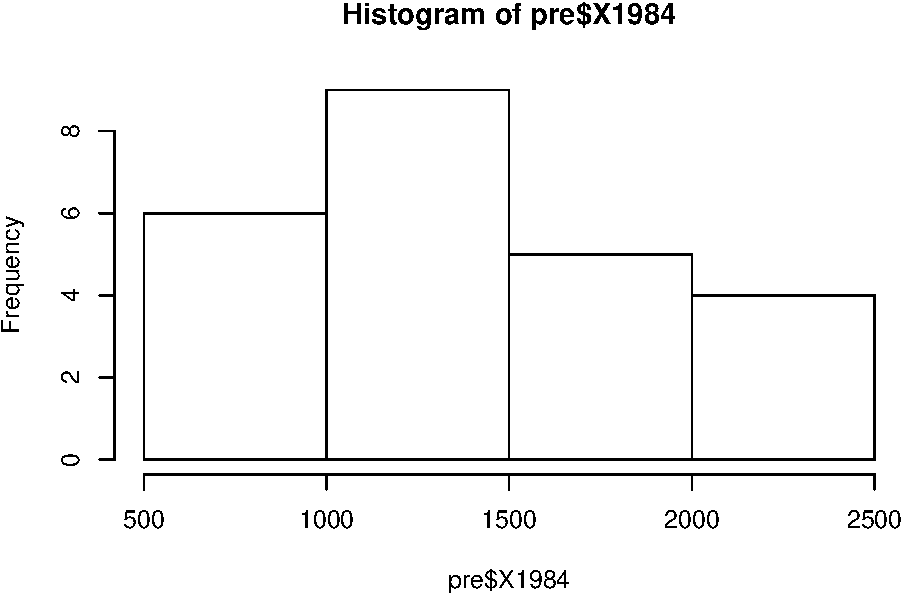
\includegraphics{proyecto_files/figure-latex/unnamed-chunk-34-1.pdf}

\begin{Shaded}
\begin{Highlighting}[]
\KeywordTok{hist}\NormalTok{(}\KeywordTok{log}\NormalTok{(pre}\OperatorTok{$}\NormalTok{X1984))}
\end{Highlighting}
\end{Shaded}

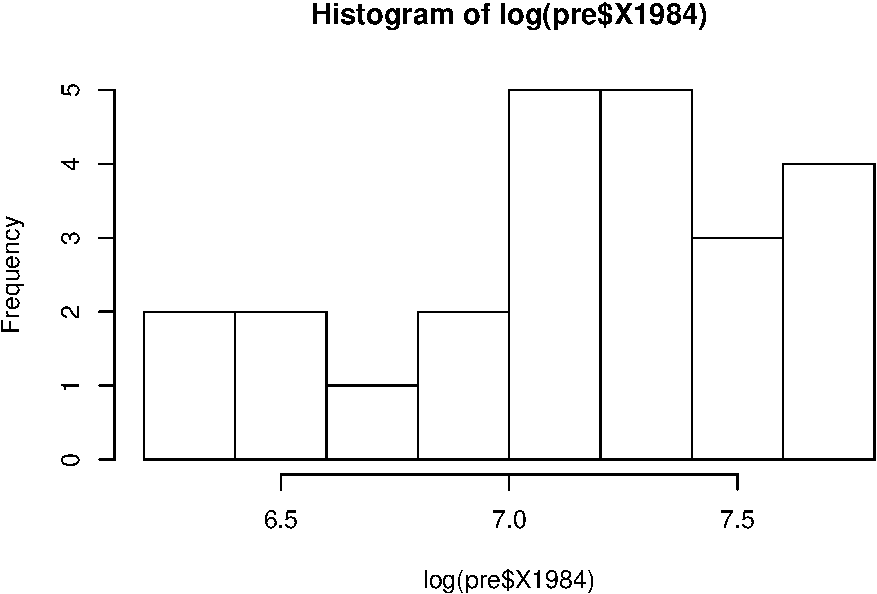
\includegraphics{proyecto_files/figure-latex/unnamed-chunk-34-2.pdf}

\begin{Shaded}
\begin{Highlighting}[]
\KeywordTok{shapiro.test}\NormalTok{(pre}\OperatorTok{$}\NormalTok{X1984)}
\end{Highlighting}
\end{Shaded}

\begin{verbatim}
## 
##  Shapiro-Wilk normality test
## 
## data:  pre$X1984
## W = 0.9436, p-value = 0.1961
\end{verbatim}

\begin{Shaded}
\begin{Highlighting}[]
\KeywordTok{shapiro.test}\NormalTok{(}\KeywordTok{log}\NormalTok{(pre}\OperatorTok{$}\NormalTok{X1984))}
\end{Highlighting}
\end{Shaded}

\begin{verbatim}
## 
##  Shapiro-Wilk normality test
## 
## data:  log(pre$X1984)
## W = 0.93376, p-value = 0.1183
\end{verbatim}

\begin{Shaded}
\begin{Highlighting}[]
\NormalTok{pre1984 <-}\StringTok{ }\KeywordTok{na.omit}\NormalTok{(pre[,}\KeywordTok{c}\NormalTok{(}\StringTok{'Estación', '}\NormalTok{X1984}\StringTok{')])}
\StringTok{pre1984$X1984log <- log(pre1984$X1984)}
\StringTok{pre1984}
\end{Highlighting}
\end{Shaded}

\begin{verbatim}
## Simple feature collection with 24 features and 3 fields
## geometry type:  POINT
## dimension:      XY
## bbox:           xmin: 215264.1 ymin: 1999092 xmax: 566794.7 ymax: 2197035
## epsg (SRID):    32619
## proj4string:    +proj=utm +zone=19 +datum=WGS84 +units=m +no_defs
## First 10 features:
##            Estación  X1984                     geom X1984log
## 1          Barahona  584.1 POINT (277900.2 2013585) 6.370072
## 2         Bayaguana 1645.6 POINT (433242.1 2073284) 7.405860
## 3           Cabrera 1888.7   POINT (405636 2171119) 7.543644
## 5  Gaspar Hernández 2208.8 POINT (363678.2 2169619) 7.700205
## 6       Hondo Valle 1796.6 POINT (215264.1 2071669) 7.493651
## 7            Jimaní  641.5 POINT (221953.7 2045651) 6.463809
## 8          La Unión 1499.4 POINT (337592.1 2184559) 7.312820
## 9           La Vega 1550.1 POINT (338847.1 2125548) 7.346075
## 10     Las Américas  954.9 POINT (429562.7 2038222) 6.861607
## 11             Moca 1256.8 POINT (342475.8 2143891) 7.136324
\end{verbatim}

\begin{Shaded}
\begin{Highlighting}[]
\KeywordTok{ggplot}\NormalTok{() }\OperatorTok{+}
\StringTok{  }\KeywordTok{geom_sf}\NormalTok{(}\DataTypeTok{data =}\NormalTok{ prov, }\DataTypeTok{fill =} \StringTok{'white'}\NormalTok{) }\OperatorTok{+}
\StringTok{  }\KeywordTok{geom_sf}\NormalTok{(}\DataTypeTok{data =}\NormalTok{ pre1984, }\KeywordTok{aes}\NormalTok{(}\DataTypeTok{col =}\NormalTok{ X1984log), }\DataTypeTok{size =} \DecValTok{6}\NormalTok{) }\OperatorTok{+}
\StringTok{  }\KeywordTok{scale_colour_gradient}\NormalTok{(}\DataTypeTok{low=}\StringTok{"#deebf7"}\NormalTok{, }\DataTypeTok{high=}\StringTok{"#3182bd"}\NormalTok{) }\OperatorTok{+}
\StringTok{  }\KeywordTok{geom_sf_text}\NormalTok{(}\DataTypeTok{data =}\NormalTok{ prov, }\KeywordTok{aes}\NormalTok{(}\DataTypeTok{label=}\NormalTok{TOPONIMIA), }\DataTypeTok{check_overlap =}\NormalTok{ T, }\DataTypeTok{size =} \DecValTok{2}\NormalTok{) }\OperatorTok{+}
\StringTok{  }\KeywordTok{geom_sf_text}\NormalTok{(}\DataTypeTok{data =}\NormalTok{ pre1984, }\KeywordTok{aes}\NormalTok{(}\DataTypeTok{label=}\NormalTok{Estación), }\DataTypeTok{check_overlap =}\NormalTok{ T, }\DataTypeTok{size =} \FloatTok{1.5}\NormalTok{) }\OperatorTok{+}
\StringTok{  }\KeywordTok{theme_bw}\NormalTok{()}
\end{Highlighting}
\end{Shaded}

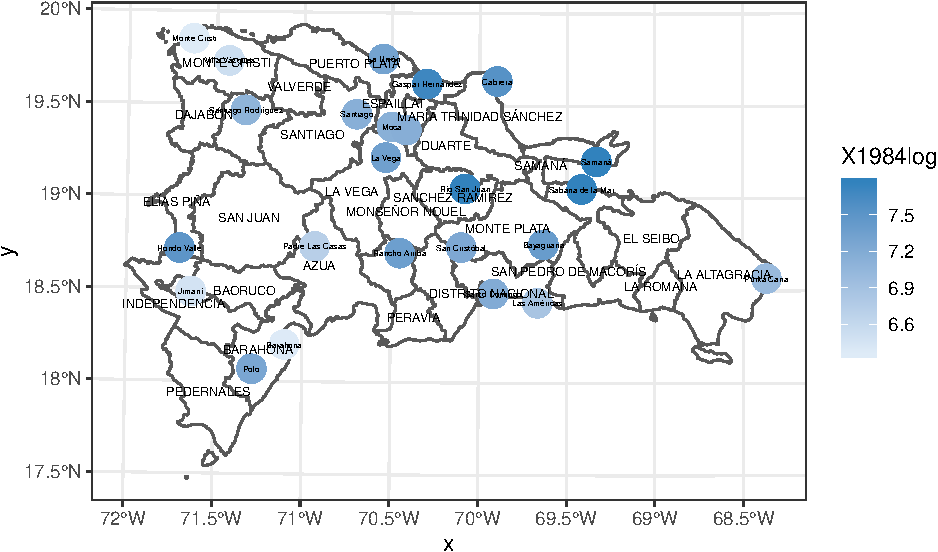
\includegraphics{proyecto_files/figure-latex/unnamed-chunk-34-3.pdf}

\section{Variograma Muestral}\label{variograma-muestral}

\begin{Shaded}
\begin{Highlighting}[]
\NormalTok{v84 <-}\StringTok{ }\KeywordTok{variogram}\NormalTok{(X1984log}\OperatorTok{~}\DecValTok{1}\NormalTok{, pre1984)}
\NormalTok{v84}
\end{Highlighting}
\end{Shaded}

\begin{verbatim}
##    np       dist        gamma dir.hor dir.ver   id
## 1   1   8896.559 0.0001451891       0       0 var1
## 2   7  22355.182 0.1409122950       0       0 var1
## 3  10  31825.181 0.0897696021       0       0 var1
## 4   7  40532.384 0.0213506432       0       0 var1
## 5   7  50078.452 0.1392497557       0       0 var1
## 6  11  58726.449 0.0858644596       0       0 var1
## 7  10  67654.274 0.0508815566       0       0 var1
## 8   9  77223.824 0.0938905087       0       0 var1
## 9  22  85005.467 0.1417784481       0       0 var1
## 10  8  93541.089 0.2076362594       0       0 var1
## 11 10 103151.699 0.0922481043       0       0 var1
## 12 16 112478.334 0.1520365569       0       0 var1
## 13 15 120178.255 0.1911321379       0       0 var1
## 14 14 128628.216 0.1994019648       0       0 var1
\end{verbatim}

\begin{Shaded}
\begin{Highlighting}[]
\KeywordTok{plot}\NormalTok{(v84, }\DataTypeTok{plot.numbers =}\NormalTok{ T)}
\end{Highlighting}
\end{Shaded}

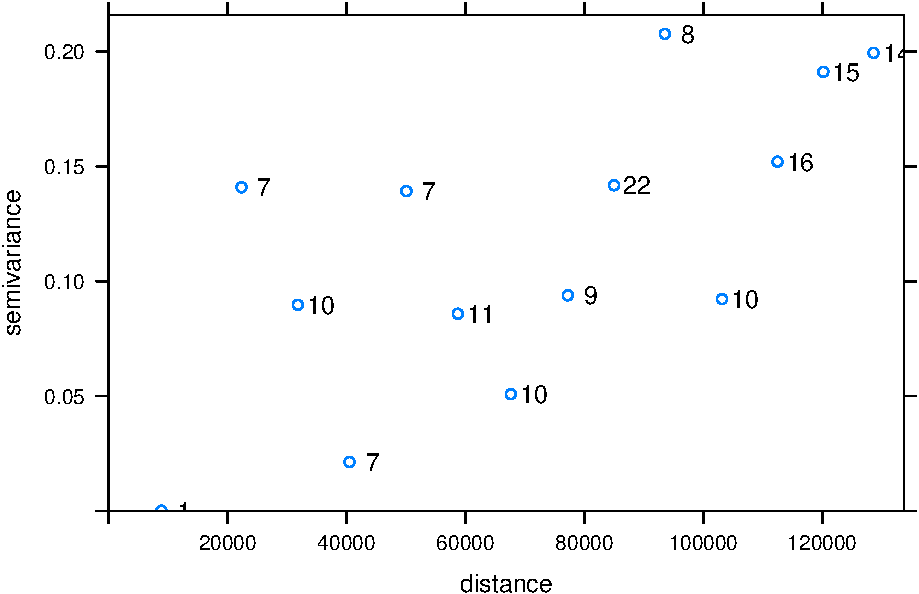
\includegraphics{proyecto_files/figure-latex/unnamed-chunk-35-1.pdf}

\section{Variograma Modelo}\label{variograma-modelo}

\begin{Shaded}
\begin{Highlighting}[]
\NormalTok{v84_m <-}\StringTok{ }\KeywordTok{fit.variogram}\NormalTok{(v84, }\KeywordTok{vgm}\NormalTok{(}\DataTypeTok{model =} \StringTok{"Sph"}\NormalTok{, }\DataTypeTok{range =} \DecValTok{50000}\NormalTok{))}
\end{Highlighting}
\end{Shaded}

\begin{verbatim}
## Warning in fit.variogram(v84, vgm(model = "Sph", range = 50000)): No
## convergence after 200 iterations: try different initial values?
\end{verbatim}

\begin{Shaded}
\begin{Highlighting}[]
\NormalTok{v84_m}
\end{Highlighting}
\end{Shaded}

\begin{verbatim}
##   model     psill    range
## 1   Sph 0.1080253 31096.24
\end{verbatim}

\begin{Shaded}
\begin{Highlighting}[]
\KeywordTok{plot}\NormalTok{(v84, v84_m, }\DataTypeTok{plot.numbers =}\NormalTok{ T)}
\end{Highlighting}
\end{Shaded}

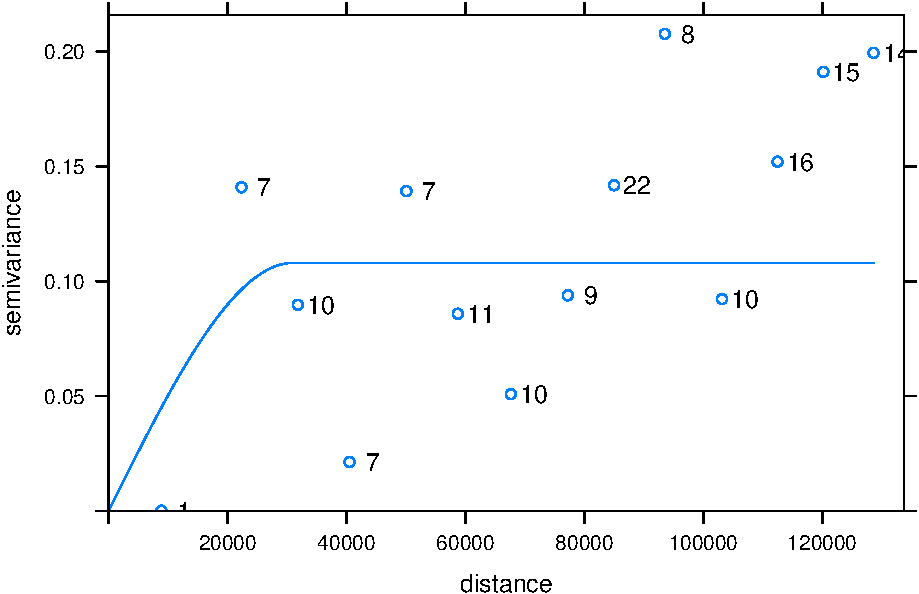
\includegraphics{proyecto_files/figure-latex/unnamed-chunk-36-1.pdf}

\begin{Shaded}
\begin{Highlighting}[]
\NormalTok{v84_m2 <-}\StringTok{ }\KeywordTok{fit.variogram}\NormalTok{(v84, }\KeywordTok{vgm}\NormalTok{(}\DataTypeTok{model =} \StringTok{"Exp"}\NormalTok{, }\DataTypeTok{range =} \DecValTok{50000}\NormalTok{))}
\NormalTok{v84_m2}
\end{Highlighting}
\end{Shaded}

\begin{verbatim}
##   model     psill    range
## 1   Exp 0.1263315 21115.94
\end{verbatim}

\begin{Shaded}
\begin{Highlighting}[]
\KeywordTok{plot}\NormalTok{(v84, v84_m2, }\DataTypeTok{plot.numbers =}\NormalTok{ T)}
\end{Highlighting}
\end{Shaded}

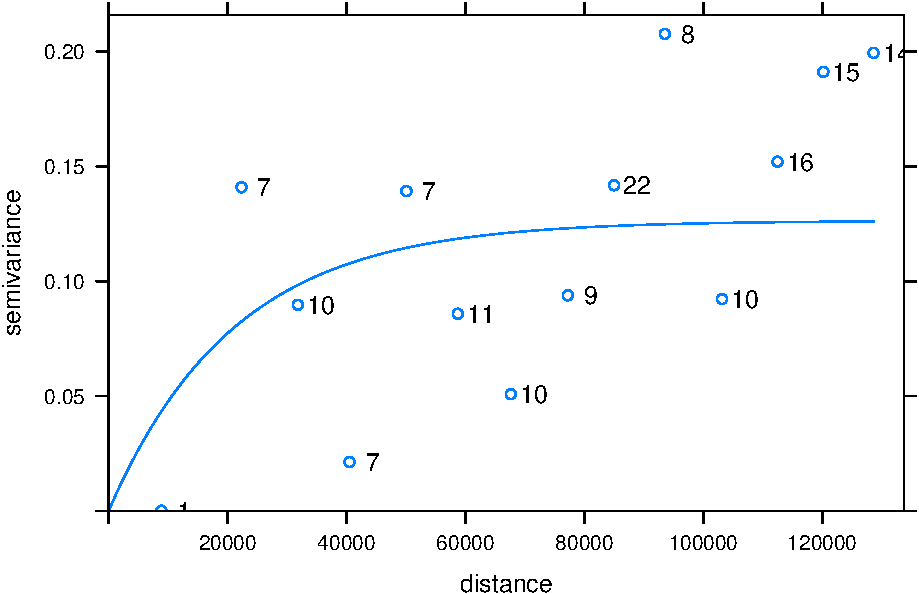
\includegraphics{proyecto_files/figure-latex/unnamed-chunk-36-2.pdf}

\begin{Shaded}
\begin{Highlighting}[]
\NormalTok{v84_m3 <-}\StringTok{ }\KeywordTok{fit.variogram}\NormalTok{(v84, }\KeywordTok{vgm}\NormalTok{(}\DataTypeTok{model =} \StringTok{"Gau"}\NormalTok{, }\DataTypeTok{range =} \DecValTok{50000}\NormalTok{))}
\end{Highlighting}
\end{Shaded}

\begin{verbatim}
## Warning in fit.variogram(v84, vgm(model = "Gau", range = 50000)): No
## convergence after 200 iterations: try different initial values?
\end{verbatim}

\begin{Shaded}
\begin{Highlighting}[]
\NormalTok{v84_m3}
\end{Highlighting}
\end{Shaded}

\begin{verbatim}
##   model     psill    range
## 1   Gau 0.1145856 19664.54
\end{verbatim}

\begin{Shaded}
\begin{Highlighting}[]
\KeywordTok{plot}\NormalTok{(v84, v84_m3, }\DataTypeTok{plot.numbers =}\NormalTok{ T)}
\end{Highlighting}
\end{Shaded}

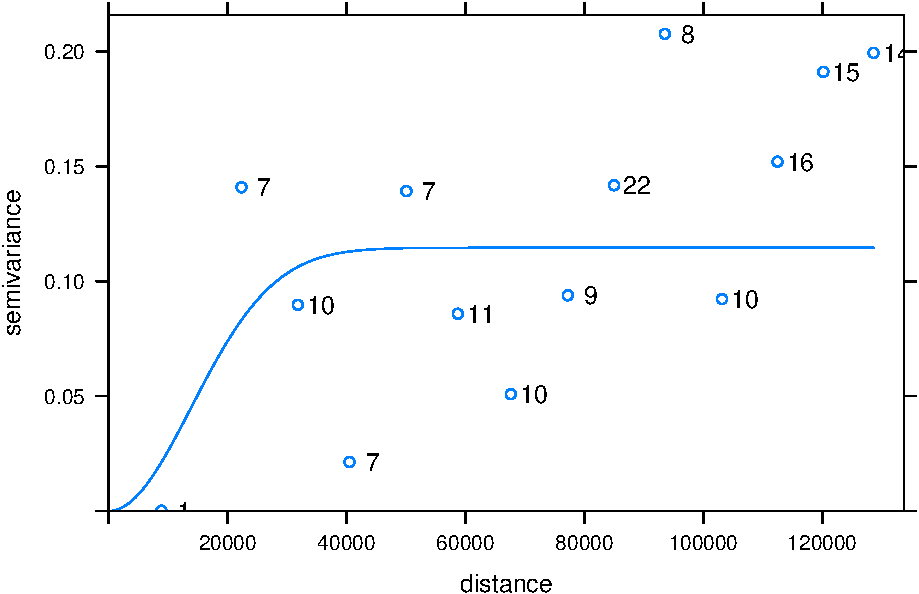
\includegraphics{proyecto_files/figure-latex/unnamed-chunk-36-3.pdf}

\begin{Shaded}
\begin{Highlighting}[]
\KeywordTok{attr}\NormalTok{(v84_m, }\StringTok{'SSErr'}\NormalTok{)}
\end{Highlighting}
\end{Shaded}

\begin{verbatim}
## [1] 1.29738e-10
\end{verbatim}

\begin{Shaded}
\begin{Highlighting}[]
\KeywordTok{attr}\NormalTok{(v84_m2, }\StringTok{'SSErr'}\NormalTok{)}
\end{Highlighting}
\end{Shaded}

\begin{verbatim}
## [1] 1.393237e-10
\end{verbatim}

\begin{Shaded}
\begin{Highlighting}[]
\KeywordTok{attr}\NormalTok{(v84_m3, }\StringTok{'SSErr'}\NormalTok{)}
\end{Highlighting}
\end{Shaded}

\begin{verbatim}
## [1] 1.292629e-10
\end{verbatim}

\section{Interpolación por kriging
ordinario}\label{interpolaciuxf3n-por-kriging-ordinario}

\begin{Shaded}
\begin{Highlighting}[]
\NormalTok{crsdestino <-}\StringTok{ }\DecValTok{32619}
\NormalTok{grd <-}\StringTok{ }\KeywordTok{st_bbox}\NormalTok{(prov) }\OperatorTok
\StringTok{  }\KeywordTok{st_as_stars}\NormalTok{(}\DataTypeTok{dx =} \DecValTok{5000}\NormalTok{) }\OperatorTok\StringTok{ }
\StringTok{  }\KeywordTok{st_set_crs}\NormalTok{(crsdestino) }\OperatorTok
\StringTok{  }\KeywordTok{st_crop}\NormalTok{(prov)}

\KeywordTok{plot}\NormalTok{(grd)}
\end{Highlighting}
\end{Shaded}

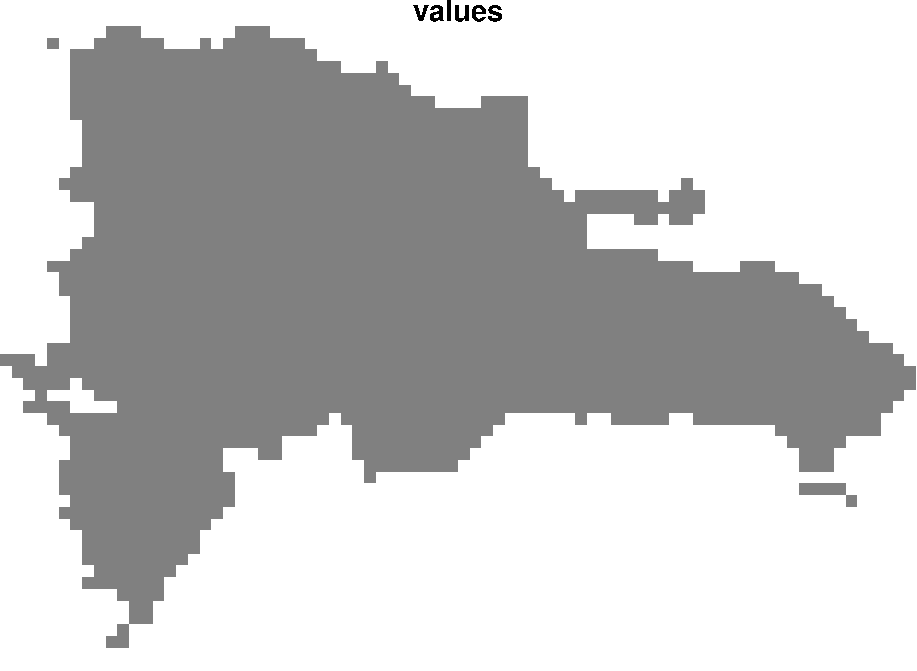
\includegraphics{proyecto_files/figure-latex/unnamed-chunk-37-1.pdf}

\begin{Shaded}
\begin{Highlighting}[]
\NormalTok{k <-}\StringTok{ }\KeywordTok{krige}\NormalTok{(}\DataTypeTok{formula =}\NormalTok{ X1984log}\OperatorTok{~}\DecValTok{1}\NormalTok{, }\DataTypeTok{locations =}\NormalTok{ pre1984, }\DataTypeTok{newdata =}\NormalTok{ grd, }\DataTypeTok{model =}\NormalTok{ v84_m2) }
\end{Highlighting}
\end{Shaded}

\begin{verbatim}
## [using ordinary kriging]
\end{verbatim}

\begin{Shaded}
\begin{Highlighting}[]
\NormalTok{k}
\end{Highlighting}
\end{Shaded}

\begin{verbatim}
## stars object with 2 dimensions and 2 attributes
## attribute(s):
##    var1.pred       var1.var      
##  Min.   :6.387   Min.   :0.0062  
##  1st Qu.:7.069   1st Qu.:0.0894  
##  Median :7.149   Median :0.1100  
##  Mean   :7.154   Mean   :0.1031  
##  3rd Qu.:7.263   3rd Qu.:0.1218  
##  Max.   :7.733   Max.   :0.1337  
##  NA's   :2361    NA's   :2361    
## dimension(s):
##   from to  offset delta                       refsys point values    
## x    1 78  182216  5000 +proj=utm +zone=19 +datum...    NA   NULL [x]
## y    1 55 2205216 -5000 +proj=utm +zone=19 +datum...    NA   NULL [y]
\end{verbatim}

\begin{Shaded}
\begin{Highlighting}[]
\KeywordTok{plot}\NormalTok{(k)}
\end{Highlighting}
\end{Shaded}

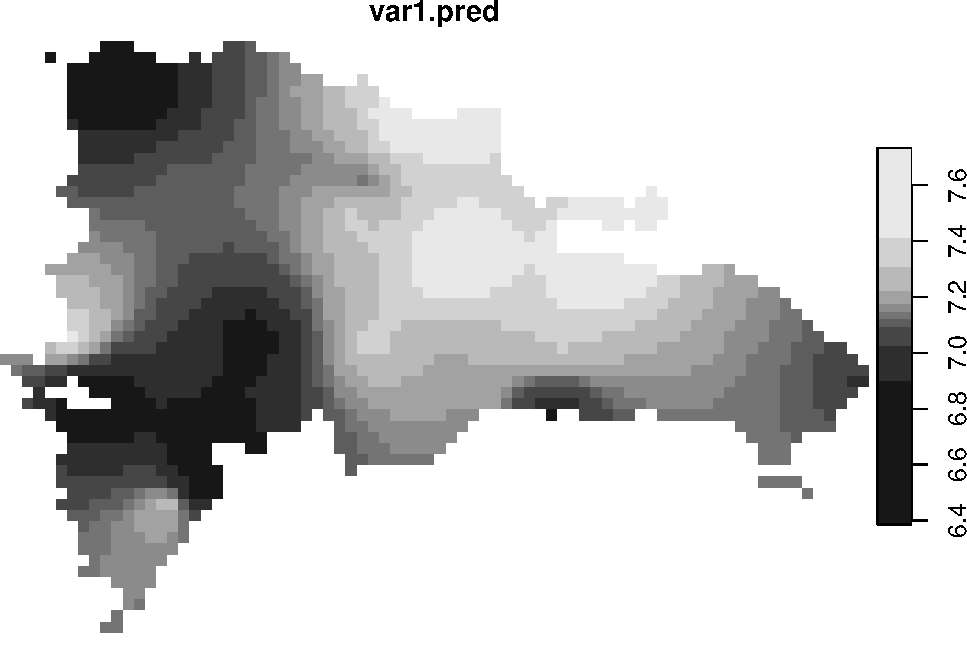
\includegraphics{proyecto_files/figure-latex/unnamed-chunk-37-2.pdf}

\begin{Shaded}
\begin{Highlighting}[]
\KeywordTok{ggplot}\NormalTok{() }\OperatorTok{+}
\StringTok{  }\KeywordTok{geom_stars}\NormalTok{(}\DataTypeTok{data =}\NormalTok{ k, }\KeywordTok{aes}\NormalTok{(}\DataTypeTok{fill =}\NormalTok{ var1.pred, }\DataTypeTok{x =}\NormalTok{ x, }\DataTypeTok{y =}\NormalTok{ y)) }\OperatorTok{+}\StringTok{ }
\StringTok{  }\KeywordTok{scale_fill_gradient}\NormalTok{(}\DataTypeTok{low=}\StringTok{"#deebf7"}\NormalTok{, }\DataTypeTok{high=}\StringTok{"#3182bd"}\NormalTok{) }\OperatorTok{+}
\StringTok{  }\KeywordTok{geom_sf}\NormalTok{(}\DataTypeTok{data =} \KeywordTok{st_cast}\NormalTok{(prov, }\StringTok{"MULTILINESTRING"}\NormalTok{)) }\OperatorTok{+}
\StringTok{  }\KeywordTok{geom_sf}\NormalTok{(}\DataTypeTok{data =}\NormalTok{ pre1984) }\OperatorTok{+}
\StringTok{  }\KeywordTok{geom_sf_text}\NormalTok{(}\DataTypeTok{data =}\NormalTok{ prov, }\KeywordTok{aes}\NormalTok{(}\DataTypeTok{label=}\NormalTok{TOPONIMIA), }\DataTypeTok{check_overlap =}\NormalTok{ T, }\DataTypeTok{size =} \DecValTok{2}\NormalTok{) }\OperatorTok{+}
\StringTok{  }\KeywordTok{theme_bw}\NormalTok{()}
\end{Highlighting}
\end{Shaded}

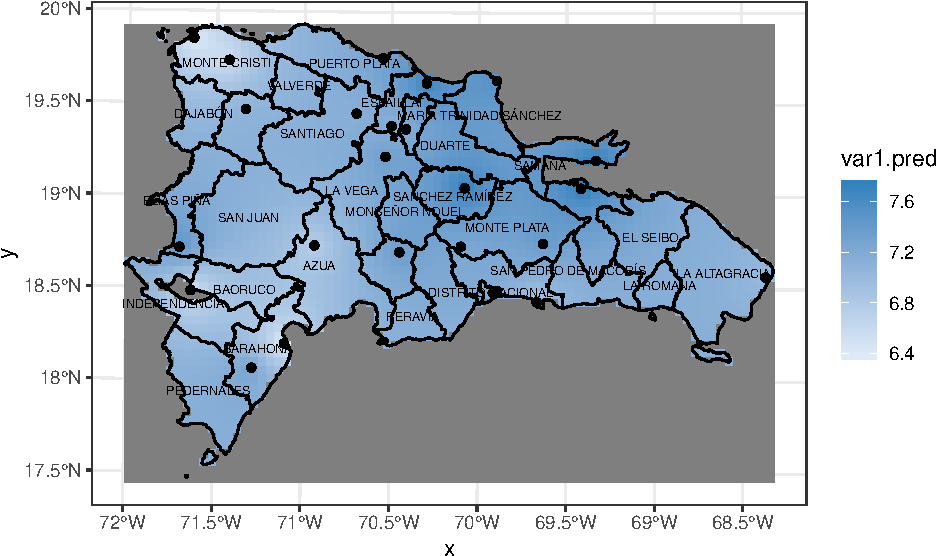
\includegraphics{proyecto_files/figure-latex/unnamed-chunk-37-3.pdf}

\begin{Shaded}
\begin{Highlighting}[]
\KeywordTok{ggplot}\NormalTok{() }\OperatorTok{+}
\StringTok{  }\KeywordTok{geom_stars}\NormalTok{(}\DataTypeTok{data =} \KeywordTok{exp}\NormalTok{(k), }\KeywordTok{aes}\NormalTok{(}\DataTypeTok{fill =}\NormalTok{ var1.pred, }\DataTypeTok{x =}\NormalTok{ x, }\DataTypeTok{y =}\NormalTok{ y)) }\OperatorTok{+}\StringTok{ }
\StringTok{  }\KeywordTok{scale_fill_gradient}\NormalTok{(}\DataTypeTok{low=}\StringTok{"#deebf7"}\NormalTok{, }\DataTypeTok{high=}\StringTok{"#3182bd"}\NormalTok{, }\DataTypeTok{trans =} \StringTok{'log10'}\NormalTok{) }\OperatorTok{+}
\StringTok{  }\KeywordTok{geom_sf}\NormalTok{(}\DataTypeTok{data =} \KeywordTok{st_cast}\NormalTok{(prov, }\StringTok{"MULTILINESTRING"}\NormalTok{)) }\OperatorTok{+}
\StringTok{  }\KeywordTok{geom_sf}\NormalTok{(}\DataTypeTok{data =}\NormalTok{ pre1984) }\OperatorTok{+}
\StringTok{  }\KeywordTok{geom_sf_text}\NormalTok{(}\DataTypeTok{data =}\NormalTok{ prov, }\KeywordTok{aes}\NormalTok{(}\DataTypeTok{label=}\NormalTok{TOPONIMIA), }\DataTypeTok{check_overlap =}\NormalTok{ T, }\DataTypeTok{size =} \DecValTok{2}\NormalTok{) }\OperatorTok{+}
\StringTok{  }\KeywordTok{theme_bw}\NormalTok{()}
\end{Highlighting}
\end{Shaded}

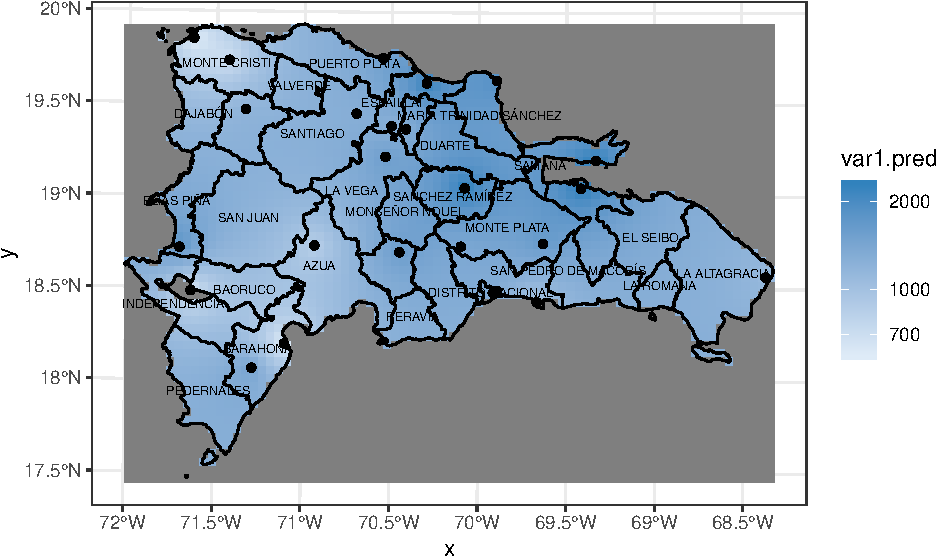
\includegraphics{proyecto_files/figure-latex/unnamed-chunk-37-4.pdf} \#
Referencias

\url{https://censo2010.one.gob.do/}




\newpage
\singlespacing 
\end{document}
